%%%%%%%%%%%%%%%%%%%%%%%%%%%%%%%%%%%%%%%%%
% Arsclassica Article
% LaTeX Template
% Version 1.1 (1/8/17)
%
% This template has been downloaded from:
% http://www.LaTeXTemplates.com
%
% Original author:
% Lorenzo Pantieri (http://www.lorenzopantieri.net) with extensive modifications by:
% Vel (vel@latextemplates.com)
%
% License:
% CC BY-NC-SA 3.0 (http://creativecommons.org/licenses/by-nc-sa/3.0/)
%
%%%%%%%%%%%%%%%%%%%%%%%%%%%%%%%%%%%%%%%%%

%----------------------------------------------------------------------------------------
%	PACKAGES AND OTHER DOCUMENT CONFIGURATIONS
%----------------------------------------------------------------------------------------

\documentclass[
10pt, % Main document font size
a4paper, % Paper type, use 'letterpaper' for US Letter paper
oneside, % One page layout (no page indentation)
%twoside, % Two page layout (page indentation for binding and different headers)
headinclude,footinclude, % Extra spacing for the header and footer
BCOR5mm, % Binding correction
]{scrartcl}

%%%%%%%%%%%%%%%%%%%%%%%%%%%%%%%%%%%%%%%%%
% Arsclassica Article
% Structure Specification File
%
% This file has been downloaded from:
% http://www.LaTeXTemplates.com
%
% Original author:
% Lorenzo Pantieri (http://www.lorenzopantieri.net) with extensive modifications by:
% Vel (vel@latextemplates.com)
%
% License:
% CC BY-NC-SA 3.0 (http://creativecommons.org/licenses/by-nc-sa/3.0/)
%
%%%%%%%%%%%%%%%%%%%%%%%%%%%%%%%%%%%%%%%%%

%----------------------------------------------------------------------------------------
%	REQUIRED PACKAGES
%----------------------------------------------------------------------------------------

\usepackage[
nochapters, % Turn off chapters since this is an article        
beramono, % Use the Bera Mono font for monospaced text (\texttt)
eulermath,% Use the Euler font for mathematics
pdfspacing, % Makes use of pdftex’ letter spacing capabilities via the microtype package
dottedtoc % Dotted lines leading to the page numbers in the table of contents
]{classicthesis} % The layout is based on the Classic Thesis style

\usepackage{arsclassica} % Modifies the Classic Thesis package

\usepackage[T1]{fontenc} % Use 8-bit encoding that has 256 glyphs

\usepackage[utf8]{inputenc} % Required for including letters with accents

\usepackage{graphicx} % Required for including images
\graphicspath{{Figures/}} % Set the default folder for images

\usepackage{enumitem} % Required for manipulating the whitespace between and within lists

\usepackage{lipsum} % Used for inserting dummy 'Lorem ipsum' text into the template

\usepackage{subfig} % Required for creating figures with multiple parts (subfigures)

\usepackage{amsmath,amssymb,amsthm} % For including math equations, theorems, symbols, etc

\usepackage{varioref} % More descriptive referencing

\usepackage{booktabs} 

\usepackage{geometry}
\usepackage{multirow}
\usepackage{booktabs}
\usepackage{array}

\usepackage{float}
\usepackage{hyperref}
\usepackage{xcolor}
%----------------------------------------------------------------------------------------
%	THEOREM STYLES
%---------------------------------------------------------------------------------------

\theoremstyle{definition} % Define theorem styles here based on the definition style (used for definitions and examples)
\newtheorem{definition}{Definition}

\theoremstyle{plain} % Define theorem styles here based on the plain style (used for theorems, lemmas, propositions)
\newtheorem{theorem}{Theorem}

\theoremstyle{remark} % Define theorem styles here based on the remark style (used for remarks and notes)

%----------------------------------------------------------------------------------------
%	HYPERLINKS
%---------------------------------------------------------------------------------------

\hypersetup{
%draft, % Uncomment to remove all links (useful for printing in black and white)
colorlinks=true, breaklinks=true, bookmarks=true,bookmarksnumbered,
urlcolor=webbrown, linkcolor=RoyalBlue, citecolor=webgreen, % Link colors
pdftitle={}, % PDF title
pdfauthor={\textcopyright}, % PDF Author
pdfsubject={}, % PDF Subject
pdfkeywords={}, % PDF Keywords
pdfcreator={pdfLaTeX}, % PDF Creator
pdfproducer={LaTeX with hyperref and ClassicThesis} % PDF producer
} % Include the structure.tex file which specified the document structure and layout

\hyphenation{Fortran hy-phen-ation} % Specify custom hyphenation points in words with dashes where you would like hyphenation to occur, or alternatively, don't put any dashes in a word to stop hyphenation altogether

%----------------------------------------------------------------------------------------
%	TITLE AND AUTHOR(S)
%----------------------------------------------------------------------------------------

\title{\normalfont\spacedallcaps{Carry: Advancing The Future of GameFi}} % The article title

%\subtitle{Subtitle} % Uncomment to display a subtitle

\author{\spacedlowsmallcaps{ Andy Pan\textsuperscript{1}}} % The article author(s) - author affiliations need to be specified in the AUTHOR AFFILIATIONS block

\date{Feb, 2024} % An optional date to appear under the author(s)

%----------------------------------------------------------------------------------------

\begin{document}

%----------------------------------------------------------------------------------------
%	HEADERS
%----------------------------------------------------------------------------------------

\renewcommand{\sectionmark}[1]{\markright{\spacedlowsmallcaps{#1}}} % The header for all pages (oneside) or for even pages (twoside)
%\renewcommand{\subsectionmark}[1]{\markright{\thesubsection~#1}} % Uncomment when using the twoside option - this modifies the header on odd pages
\lehead{\mbox{\llap{\small\thepage\kern1em\color{halfgray} \vline}\color{halfgray}\hspace{0.5em}\rightmark\hfil}} % The header style

\pagestyle{scrheadings} % Enable the headers specified in this block

%----------------------------------------------------------------------------------------
%	TABLE OF CONTENTS & LISTS OF FIGURES AND TABLES
%----------------------------------------------------------------------------------------

\maketitle % Print the title/author/date block

\setcounter{tocdepth}{2} % Set the depth of the table of contents to show sections and subsections only

\tableofcontents % Print the table of contents

\listoffigures % Print the list of figures

% \listoftables % Print the list of tables

\let\thefootnote\relax\footnotetext{\textsuperscript{1} \textit{Principle Engineer, Singapore}}

\newpage
%----------------------------------------------------------------------------------------
%	ABSTRACT
%----------------------------------------------------------------------------------------
\section*{Abstract} % This section will not appear in the table of contents due to the star (\section*)

Carry introduces an innovative protocol tailored for the game industry, offering the potential for increased revenue for game developers and players. By replacing traditional game platforms, Carry protocol provides powerful features for building, conducting analysis in games, bridging Web2 and Web3 games, and placing in game advertisement. \\

The Carry Protocol introduces a transformative approach to integrating advertising into the world of web3 games. Through the innovative concept of slots - virtual spaces, soundscapes, or digital entities within games - it offers an unintrusive avenue for presenting advertisements. These slots, inherently tied to specific game environments, can manifest as visual displays, auditory cues, or even interactive virtual entities. Given their intrinsic value, slots are not just static elements but tradable assets within the Carry ecosystem. The paper delves deep into the mechanics of slots, elucidating their lifecycle, potential monetization strategies through auctions, and the importance of performance metrics in optimizing their impact. Moreover, the role of the Carry token and Carry fuel underpins the economic dynamics of the system, ensuring seamless transactions within the Carry marketplace. This protocol harnesses the power of blockchain and decentralized governance, promoting a balanced, sustainable, and player-centric advertising ecosystem in the game world. \\

Carry Protocol also offers a robust platform equipped with an Software Development Kit (SDK) and powerful modular tools, enabling game developers to efficiently manage and monetize digital assets such as fungible and non-fungible tokens (FTs and NFTs). The Carry SDK enables Web2 games to integrate blockchain technology easily. At the same time, Carry SDK provides a simplified mechanism for managing in-game assets and user accounts for both Web2 and Web3 games. 

%----------------------------------------------------------------------------------------
%	AUTHOR AFFILIATIONS
%----------------------------------------------------------------------------------------

% \let\thefootnote\relax\footnotetext{* \textit{Tbook, CEO, Shanghai, China}}



%----------------------------------------------------------------------------------------

\newpage % Start the article content on the second page, remove this if you have a longer abstract that goes onto the second page

%----------------------------------------------------------------------------------------
%	INTRODUCTION
%----------------------------------------------------------------------------------------

\section{Introduction}
Carry Protocol aims at building a next generation game infrastructure. The infrastructure aims to fill the gap between Web2 and Web3 games, at the same time creating a fair game economics for blockchain games to thrive as never before. Briefly, Carry introduces an innovative advertising protocol tailored for the game industry, offering the potential for increased revenue for game developers and players. By replacing traditional advertising platforms, this protocol not only enhances the advertising effectiveness for advertisers but also reduces associated costs. \\

The Carry Protocol innovatively bridges the worlds of games and advertising within the web3 space, offering a unique system for showcasing ads within virtual game environments. These advertising spaces, or "slots," are thoughtfully integrated into games, functioning like digital billboards for interactive promotions. This approach aims to create a better and healthier game advertising economics.\\

Moreover, the protocol incorporates a transparent and equitable auction system to allocate advertising space, where the market value of each slot is determined by real-time demand. This system ensures a fair and open process for all participants.\\

The Carry SDK on the side, will provide powerful infrastructure for both Web2 and Web3 games to easily integrate blockchain features. Furthermore, Carry provides adaptive data analysis module for various kinds of games to achieve strategy optimization and service evolution.


\subsection{Motivation}
In this section, we attempt to summarize the primary challenges of the current game market.
\begin{itemize}[leftmargin=*]
    \item \textbf{Failed Incentives:} The dominance of the play-to-earn dual-token economic model in many web3 games, although initially promising, has demonstrated its limitations. Due to its aggressive and singular incentive structure, it often places developers and players in positions of discordant interests, threatening the game’s longevity \cite{leonardos2020oceanic}. In the later stages of the vast majority of play-to-earn games, due to the singularity of incentive mechanisms, players can solely profit by selling their held NFT assets. Regardless of the developers’ efforts to salvage or enhance the game experience, games remain highly susceptible to entering a "death spiral" within a relatively short timeframe. 
    
    For a sustainable future, web3 games necessitate diversified economic mechanisms that foster collaborative wins among developers, players, and other stakeholders.
    
    \item \textbf{Platform Monopoly:} Developers have grown weary of the "Apple tax", which, as a giant advertisement platform, dominates the web2 advertising system and web2 monetization standards by monopolizing user data assets \cite{hovenkamp2020antitrust}. The web2 advertising ecosystem primarily comprises four key players: advertisers, media, advertising platforms, and users. Advertising platforms, by monopolizing user data assets, shape the advertising monetization landscape. However, the advancement of privacy technology and blockchain technology has provided a mature technological solution for a fairer advertising protocol \cite{stallone2023enhancing}.
 
    Both developers and users have a strong demand for a more equitable and efficient advertising ecosystem. The current dominance of giant advertising platforms has significantly impacted business and innovation efficiency.

    \item \textbf{Inability to Analyze Player Intent:} Despite the transformative potential of web3 in games, many developers operate based on speculative insights about player preferences, leading to games that either wane in popularity or serve primarily for asset arbitrage. The heart of this challenge is the absence of effective tools to analyze user behavior within Web3 games. This oversight hinders developers from truly understanding player intent \cite{abeele2020development}. Notably, games like Crypto Kitties, which introduced users to the creation and trade of in-game NFTs, underscore the vast possibilities but also the need for more nuanced player behavior insights.

    Using the crypto-native game ’Loot’ as a case study, it’s evident that following its significant traction within the NFT community, over 20 development teams have emerged with a focus on Loot. These teams are diligently working on an array of games rooted in the foundational model of Loot. However, a minimal number of these endeavors have shown tangible advancement. To solve these issues, the developers and players need to have more interaction during its lifecycle. Native features in web3, for example, predict the market, provide methods for developers to truly interact with players.
 
    As a slogan in the web3 industry goes, "onchain is the new online." Therefore, a multitude of data dimensions can now be easily captured. We need greater insights into users to enhance the efficiency of advertising and games.
\end{itemize}

\subsection{Related Works \& Projects}
The Carry Protocol operates at the intersection of blockchain technology, gaming, and digital advertising, marking a significant step forward in the evolution of Web3 gaming infrastructures. To contextualize Carry's contributions, it's essential to review existing projects and research that have paved the way for innovations in game finance (GameFi), in-game advertising, and blockchain integration within the gaming industry. This section delves into several key projects and areas of work that share thematic or technical overlap with the aims of Carry Protocol.

\subsubsection{Decentraland and Virtual Real Estate}


\href{https://decentraland.org/}{Decentraland} represents a pioneering effort in creating a decentralized virtual world, where users can buy, sell, and manage virtual real estate \cite{guidi2022social}. It stands as a hallmark example of integrating blockchain technology with digital land ownership, offering a vivid parallel to Carry's slot-based advertising model. In Decentraland, landowners have complete control over their parcels, which can be developed to display content, host games, or serve advertisements, similar to Carry's vision of in-game slots as digital real estate for ads.

\subsubsection{Axie Infinity and Play-to-Earn Model Evolution}

\href{https://axieinfinity.com/}{Axie Infinity} revolutionized the GameFi space by popularizing the play-to-earn (P2E) model, where players earn cryptocurrency rewards for gameplay achievements and trading in-game assets \cite{lai2023quantitative}. While Carry Protocol acknowledges the limitations of the early P2E models, it seeks to refine this concept by creating a more sustainable and equitable economic system for all stakeholders, emphasizing the need for diversified economic mechanisms beyond the dual-token models that Axie initially introduced.

\subsubsection{Brave Browser and Attention-Based Advertising}

The \href{https://brave.com/}{Brave Browser} and its associated Basic Attention Token (BAT) introduce a novel approach to online advertising, where users are rewarded for viewing ads \cite{trotz2019times}. This model aligns closely with Carry's ethos of fair compensation for engagement. Carry extends this philosophy into the gaming domain, proposing a system where players and developers benefit directly from ad integration, suggesting a move towards more interactive and player-focused advertising strategies within the game industry. Moreover, Carry provides a general infrastructure for both traditional and emerging (Web3) games to integrate blockchain features, which is not achieved by the Brave Browser.

\subsubsection{Enjin and Asset Tokenization}

\href{https://enjin.io/}{Enjin} has been a frontrunner in providing an ecosystem for creating, managing, and integrating tokenized digital assets into games and apps. By allowing assets to be tokenized on the blockchain, Enjin facilitates true ownership of in-game items, mirroring Carry's concept of slots as tradeable digital assets \cite{marin2023review}. This parallel underscores the broader trend towards asset tokenization in gaming, enhancing the depth and liquidity of virtual economies.

\subsubsection{The Sandbox and User-Generated Content}

The \href{https://www.sandbox.game/}{Sandbox} is a user-generated content (UGC) and gaming platform that empowers players to create, own, and monetize their gaming experiences on the Ethereum blockchain \cite{truby2020fintech}. It exemplifies the potential of blockchain to democratize content creation within virtual worlds. Carry Protocol's slot-based advertising model can be seen as an extension of this democratization, where advertising spaces become a canvas for creative expression and economic participation by developers and players alike.

\subsubsection{Aavegotchi and DAO Governance in Gaming}

\href{https://aavegotchi.com/}{Aavegotchi} stands out for its integration of decentralized finance (DeFi) principles with non-fungible tokens (NFTs) within a gaming context, governed by a Decentralized Autonomous Organization (DAO) \cite{lin2023survey}. The project highlights the potential for community-driven governance models in shaping game development and economic policies, resonating with Carry's aim to foster collaborative wins among all participants in the gaming ecosystem.

\subsubsection{Comparison Analysis}

In examining these related works and projects, it's clear that the Carry Protocol is not operating in isolation but rather building upon a rich foundation of innovation in blockchain, gaming, and digital advertising. By learning from the successes and limitations of these precedents, Carry aims to forge a new path that addresses the challenges of failed incentives, platform monopolies, and the need for deeper insights into player behavior. As the blockchain and gaming landscapes continue to evolve, projects like Carry Protocol will play a crucial role in shaping the future of digital entertainment, advertising, and community engagement.

\subsection{Contributions}
\subsubsection{Slot-based Advertising Paradigm}
At the heart of the Carry Protocol lies the innovative concept of a "slot," a transformative idea designed to bridge the worlds of advertising and on-chain games. In its essence, a slot is a unique digital real estate where advertisements can be strategically placed, integrated seamlessly into the virtual environments of games or other digital platforms.

\begin{figure}[h]
    \centering
    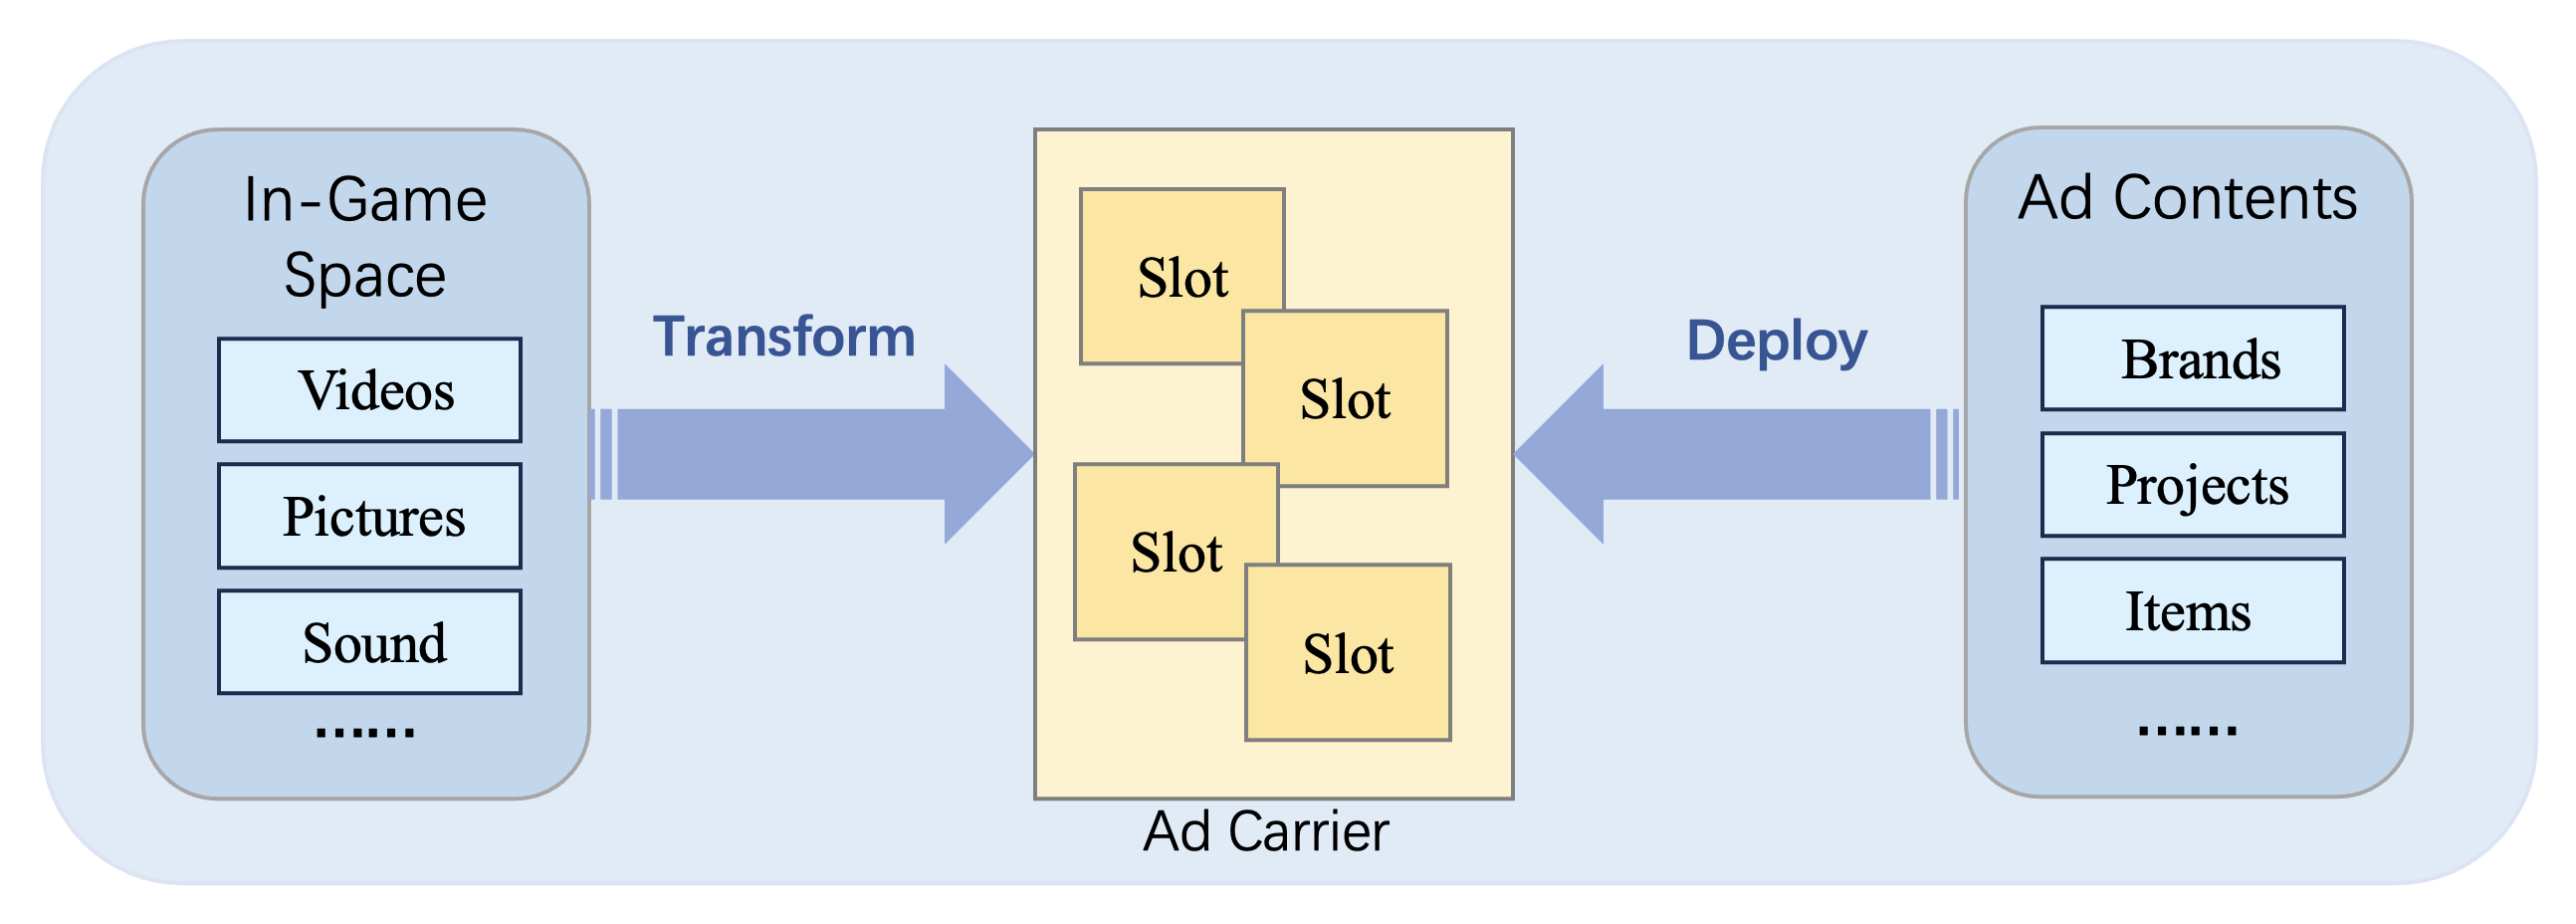
\includegraphics[width=0.7\textwidth]{Slot Design.png}
    \caption{Slot Design}
    \label{fig:slot_basic}
\end{figure}

\begin{itemize}
    \item Every slot is inherently tied to a designated game, taking forms such as visual spaces for graphics, character-specific sound effects, or virtual companions roaming the digital environment.
    \item Beyond their in-game presence, slots hold asset value and can be traded or transferred among participants.
    \item Slots can be a carrier of various types of media, videos, pictures etc.
\end{itemize}

Imagine you're playing an online game, and as you explore, you see ads on billboards or even on items like a character's backpack. These are what we call "slots" in the Carry Protocol. Think of a slot like a piece of virtual real estate where ads can live. These slots are valuable to advertisers and can be bought, sold, or traded just like other virtual items in the game.

% As shown in Figure \ref{fig:billboard}, a billboard in an RPG game is a type of virtual space that can be abstracted as slots.

% \begin{figure}[h]
%     \centering
%     \includegraphics[width=0.7\textwidth]{billboard.jpg}
%     \caption{Example of Advertisement Space in Games: when playing RPG games, the billboard can be abstracted as a slot space where advertisements can be placed on to.}
%     \label{fig:billboard}
% \end{figure}

Slots are versatile. They can show video ads, become part of the game scenery, or even be part of the outfit your character is wearing. They're designed to fit into the game naturally, so they're interesting rather than annoying.

The worth of these ad spaces can go up or down. For example, a slot right where players hang out the most could be worth a lot because more players will see the ad there, while a slot off in a quiet corner might not be as valuable.

The Carry Protocol is all about changing up the game when it comes to ads. These slots are active parts of the game that can change based on how players interact with them and what advertisers want to try. They're a new way to think about ads in games, making sure that players' experiences come first.


\subsubsection{One-Stop Game Infrastructure}

As early blockchain experts and game developers merged, there appeared to be innumerable hours spent learning seemingly nonessential concepts foreign to each other’s native skillsets. Many developers suggested that fortes were being unnecessarily overcomplicated. They needed a tool to realize their function; comprehending its mechanism should be optional education.

Without a proper foundation, an ecosystem cannot thrive. Carry SDK was developed precisely for this purpose; it’s a secure and easy-to-use library of standardized blockchain tools, or rather, a one-stop metaverse infrastructure platform for the game ecosystem. Using Carry SDK, developers no longer need to be intimidated or hindered by the security and complexity of blockchain technology. The entry threshold is lowered, and in terms of cost, eliminated. All interested gamers can expect increased playability as a result.


\subsubsection{Adaptive Game Data Analysis}
The Carry Protocol introduces an Adaptive Data Analysis Module for Web3 gaming, offering real-time insights into in-game advertising effectiveness through Performance Benchmark Metrics. This innovation enables game developers and advertisers to optimize ad placements and content dynamically, ensuring ads enhance rather than detract from the gaming experience.

By leveraging strategy simulation and comprehensive evaluation metrics, the protocol facilitates precise adjustments and targeted experiments with advertising strategies. This approach not only improves monetization strategies for developers but also ensures advertisements are engaging and relevant to the player community, marking a significant advancement in the integration of blockchain technology with the gaming industry.


\subsection{Organization}
The reminder of this Whitepaper are organized as follows. First, we introduce the proposed novel slot-based advertising paradigm, the general launching infrastructure for both Web2 and Web3 games, and the adaptive data analysis module in Section 2-4, respectively. Second, we demonstrate the designed economics and incentives for various system participants in Section 5. Third, we describe the contract-based protocol implementation and some cryptography-facilitated mechanisms in Section 6. Finally, we conclude this work in Section 7.
%----------------------------------------------------------------------------------------


\section{Proposed Novel Advertising Paradigm}

\subsection{Overview}


% Imagine playing an online game where you can own and trade parts of the game world. That's what's happening with Carry Protocol's 'slots' in new blockchain games. The Carry protocol architecture is shown in Figure \ref{fig:big_picture}.

% \begin{figure}[h]
%     \centering
%     \includegraphics[width=1\textwidth]{carryslot.jpg}
%     \caption{Carry Slot Based Advertising}
%     \label{fig:big_picture}
% \end{figure}

The Carry Protocol introduces something called "slots" in online games, which are like digital billboards or sponsored items within the game. These slots add value without getting in the way of gameplay and allow advertisers to get more bang for their buck.

Normally in games, the game makers control everything you see and use. But in these new games, players can own unique game items, like a special sword or a piece of land, which they can buy, sell, or trade. These items are called NFTs, which are like digital collectibles that you truly own.

Game developers must establish clear ownership guidelines when introducing slots as in-game advertising spaces. There are two categories of slots: those that are inherent to the game's environment (game native assets) and those that are controlled by players (player owned assets). For instance, a billboard within the game's landscape serves as a game native asset. Contrastingly, player-specific items such as character skins or pets, which are created and consequently 'minted' by players, represent player owned assets. 

% The economics of these slots, which include their creation, ownership, and value within the game's marketplace, are elaborated in Figure \ref{fig:big_picture}.

To elucidate, let's consider a hypothetical scenario. A digital realm, 'LandA', owned by 'Addr1', becomes a canvas for an advertisement. When the developer introduces a slot to this realm, it isn't just assigned to the player 'Addr1'. Instead, it's as if 'LandA' itself becomes enhanced, now comprising both the original realm and the new slot. Symbolically:

\[\text{Addr1} \rightarrow \text{Land A}\]

Transforms to:

\[\text{Addr1} \rightarrow (\text{LandA}, \text{SlotA})\]

This distinction is crucial. The slot isn't an isolated entity but rather correlates with a specific in-game asset. It isn't a generic add-on but a tailored integration. And to facilitate this tailored relationship, technologies like EIP-6220 can be leveraged, ensuring that the connection between the game asset and its corresponding slot is both seamless and efficient.

In summary, Carry Protocol is re-imagining how ads fit into video games. Instead of being annoying interruptions, they're becoming a natural part of the game's world. This setup lets game creators and players work together in new ways, making the game more engaging while also figuring out who gets to own these digital ad spaces. It's a fresh approach that could change games and advertising for the better.

\subsection{Basic Definitions}
Within the Carry Protocol, several foundational concepts drive its operation in the web3 games world. This section elucidates these essential principles, highlighting their role and importance in the Carry ecosystem.
\begin{enumerate}
    \item \textbf{Slot:} The fundamental unit within Carry, serving as the primary canvas for advertisement placements.
    \item \textbf{Slot Time:} A designated time frame for which a slot can be utilized, regulated by the Carry governance.
    \item \textbf{Auctioning:} The dynamic process by which slots' time and positioning are bid upon, determining their allocation based on market demand and value perception.
    \item \textbf{Marketplace:} A decentralized platform where slots can be traded, purchased, or leased, fostering a vibrant ecosystem around the advertisement spaces.
\end{enumerate}

\subsection{Concrete Designs}

The central tenet of the Carry Protocol hinges on the intricate lifecycle of slots. These slots are not mere placeholders but dynamic entities that embody a unique relationship with game assets and advertisements. Here's a closer look at their lifecycle:

\begin{itemize}
    \item \textbf{Creation and Initialization:} Game creators are given special slots that they can easily put into their games. Once these slots are in place, the creators or the players can start using them, turning them into one-of-a-kind digital items. 
    \item \textbf{Asset Status Management:} The protocol oversees and modifies the status of each asset, ensuring up-to-date representation within the ecosystem.
    \item \textbf{Asset Relationship Management:} The system smartly manages how different parts of the game work together, particularly when something changes. For example, when a slot stops showing an ad, the ad is no longer connected to that slot.
\end{itemize}


\subsubsection{Slot Status}
\begin{itemize}
    \item \textbf{Idle:} The slot is in a passive state, devoid of any advertisements.
    \item \textbf{Placement:} The slot is actively displaying an advertisement.
    \item \textbf{Pre-initialization:} The slot awaits proper initialization or minting, making it unowned within the ecosystem.
    \item \textbf{Initialization:} Pertains to the formal creation of a slot for a specific game asset, represented technically by the minting of the slot NFT.
\end{itemize}

\subsubsection{Slot Relationships}
Two primary relationships define a slot's existence:
\begin{itemize}
    \item \textbf{Ownership Dynamics:} Dictates the proprietorship of the slot, tracing it to either a developer, gamer, or directly linking it to a specific in-game asset. At the outset, this ownership typically aligns with a distinct game asset.
    \item \textbf{Advertisement Affiliation:} Emphasizes the bond between the slot and the advertisements it hosts. The intrinsic value of a slot is not just its mere existence, but its capacity to exhibit advertisements and, in turn, generate revenue.
\end{itemize}

\subsubsection{Slot-Ad Lifecycle}

Examining slots from an advertising temporal perspective helps understand how they accrue value in the ad ecosystem:

\begin{itemize}
    \item \textbf{Slot Placement Duration Auction:} Taking cues from platforms like OpenSea, slots undergo an auction or selection process. Unlike traditional auctions where ownership is transferred, slots are typically leased for a predetermined duration, conferring advertisement display rights without altering slot ownership.
    
    \item \textbf{Ad Content Placement:} Once a slot is chosen, it's imbued with the pertinent advertising content.
    
    \item \textbf{Value Generation:} The advertisement, once viewed or engaged with by users or gamers, starts accruing value.
    
    \item \textbf{End of Ad Cycle:} Upon reaching the designated period, the advertisement's active phase ceases, reverting the slot to its idle state.
    
    \item \textbf{Ad Effect Tracking:} This phase is earmarked for gauging the repercussions and reach of the advertisement.
    
    \item \textbf{Ad Settlement:} Beyond the initial fee amassed during the auction, any supplementary value spawned by the advertisement's efficacy is settled at this juncture.
\end{itemize}

\subsubsection{Actions on Slots}
Several actions can be taken on a slot, determining its trajectory and interaction with ads:

\begin{itemize}
    \item \textbf{Ad Placement:} Assigning a specific advertisement to the slot for display.
    
    \item \textbf{Ad Removal:} Extracting the currently showcased advertisement from the slot, returning it to a vacant state.
    
    \item \textbf{Transfer of Rights:} Conveying the privileges or ownership of the slot to another entity.
    
    \item \textbf{Slot Exchange:} Engaging in transactions to exchange slots with other participants.
\end{itemize}


\subsubsection{Placement Strategy}
The strategy of placement ads onto slots determines how slots accrue value and relevance within the game ecosystem. As developers and advertisers navigate this space, optimizing placement strategies ensures slots' maximum potential is realized. 

Carry provides the following built in strategies:
\begin{itemize}
    \item \textbf{Distinct Time Allocation:} Slots are auctioned for exclusive, well-defined time periods.
    
    \item \textbf{Periodic Time Allocation:} Slots are systematically scheduled for recurring durations.
    
    \item \textbf{Enduring Lease:} The slot is granted on a long-term basis to a specific party. Nonetheless, the lessee has the prerogative to auction this lease in the Carry marketplace.
\end{itemize}




\subsection{Governance Mechanism}

Imagine Carry Governance as the manager of a digital billboard. It matches ads with the right spots in the virtual game world, ensuring that everything fits together nicely and the game experience stays enjoyable and cohesive. Carry governance includes the following functions:

\begin{itemize}
    \item \textbf{Slot Allocation Governance:} Determines and assigns specific virtual spaces for advertisement displays.
    
    \item \textbf{Content-Slot Matching:} Regulates and ensures the relevant advertisement content is mapped to its corresponding slot.

    \item \textbf{Ad Lifecycle Management:} Governs the duration and lifecycle of an advertisement within a slot.

    \item \textbf{Ad Quality Oversight:} Establishes standards and ensures displayed advertisements meet quality and relevance criteria.
    
    \item \textbf{User Feedback Integration:} Incorporates feedback mechanisms and uses player responses to refine ad placements.

    \item \textbf{Dispute Resolution:} Manages and resolves conflicts that may arise in terms of slot assignments or advertisement displays.
\end{itemize}



\subsection{Ad Settlement Mechanism}

Beyond the foundational fee secured during the auction phase, any additional value derived from the ad's performance is settled. The settlement mechanism can be divided into:

\begin{enumerate}
    \item \textbf{Basic Placement Fee (\( BPF \))}: 
    \begin{equation}
    \text{Fee} = BPF \times t
    \end{equation}
    where \( t \) is the actual duration of the ad placement.

    \item \textbf{Performance-based Incentives (\( PM \))}: Depending on the agreement, this could be:
    \begin{itemize}
        \item \textbf{CPS (Cost Per Sale)}: For on-chain businesses, e.g., NFT sales.
        \item \textbf{CPA (Cost Per Acquisition)}: Based on user metrics.
        \item \textbf{CPL (Cost Per Liquidity)}: In scenarios like DeFi, based on staked asset value.
        \item \textbf{CPI (Cost Per Installation)}: Metrics based on app installations.
    \end{itemize}
\end{enumerate}

Ultimately, the revenue (\( R \)) for a slot owner is:
\begin{equation}
R = A \times (BPF \times t) + B \times \Sigma PM \times \Sigma PR
\end{equation}
where \( PR \) represents the Performance Ratios, and \( A \) and \( B \) are coefficients. Slot owners can adjust these coefficients to maximize their returns.

% \subsection{Carry Marketplace}
% Carry provides its own marketplace for asset trading/auctioning. These assets include:
% \begin{itemize}
%     \item Advertisement Slots
%     \item NFTs
%     \item NFTs that can be used as advertisement content
%     \item Carry token
%     \item Crypto assets like ETH and BTC etc.
% \end{itemize}

% Assets can be traded with each other on the Carry marketplace. Slots can be traded through this process. Slot time, based on the strategy, can be auctioned/traded on the Carry marketplace as well. 

% \subsubsection{Slot Auction Mechanism}


% In the Carry Protocol, slots are like prime digital real estate for ads within games. They are auctioned off to the highest bidder, similar to how you might bid for a popular item on eBay. But instead of buying the slots, advertisers rent them for a certain time. This way, they get to show their ads in the game without owning the slots permanently.

% % We suggest using a Dutch auction for selling ad space. Here's how it works: the price for advertising starts high and drops over time until someone agrees to pay. Advertisers watch the price fall and jump in when they think the price is right for the value they’ll get. This makes the selling process fast and fair because it matches what advertisers are willing to pay with what game developers expect for their ad spaces.

% % \begin{figure}[h]
% %     \centering
% %     \includegraphics[width=0.8\textwidth]{equilibrium.jpg}
% %     \caption{Equilibrium of Slot Pricing}
% %     \label{fig:equilibrium}
% % \end{figure}


% Here's a closer look at the process:
% \begin{itemize}
%     \item The slot owner (or their agent) sets an initial price for each slot placement duration. Ideally, this price is higher than the last traded price for the same slot duration.
%     \item Given the slot owner's preference for filling their slot durations, the price for the slot placement duration progressively drops over time, urging advertisers to place their bids quickly.
%     \item Advertisers monitor the pricing trend of the slot placement duration. Failing to bid in time and missing out to other bidders means losing an advertising opportunity. Hence, advertisers are inclined to bid once the price seems reasonable.
%     \item Slot owners (or agents) have a reserve price for their slot placement durations. If bids fall below this threshold, the auction becomes void and needs a restart.
% \end{itemize}



% \subsection{Slot Lifecycle}


% In a web3 game, a "slot" is essentially a spot where ads can go, chosen when the game is being made. For instance, in a shooting game, ads could appear as graffiti on a virtual wall. Who owns this ad space depends on where it is. If it's part of the game's environment, like the wall, it's owned by the game's creators. But if it's tied to a player's character, like a logo on a shirt, then the player owns it.

% The owner of a slot can decide to use it for ads themselves or offer it up to others by selling or renting it out through a marketplace. This way, slots become a flexible tool for advertising in the game world.




\section{Data Analysis Module for Games}

Blockchain games combine elements of traditional gaming with features of decentralized finance to create a new gaming and economic experience. In this context, on-chain data analysis becomes particularly important as it can offer insights into player behavior, asset liquidity, economic activities, and the health of the gaming ecosystem. Data analysis can bring several key advantages to GameFi projects:
\begin{itemize}
    \item \textbf{Transparency and Verifiability:} Since all transactions and activities are recorded on the blockchain, data analysis can provide fully transparent and verifiable insights into player behavior and economic activities.
\item \textbf{Player Behavior Insights:} Analyzing on-chain data can reveal player preferences, engagement patterns, and behavioral trends, helping developers optimize game design and enhance player experience.
\item \textbf{Economic and Asset Analysis:} Monitoring and analyzing the creation, trading, and liquidity of in-game assets allows developers to better manage the game's economy, preventing inflation or asset value collapse.
\item \textbf{Community and Ecosystem Health:} On-chain data analysis helps assess community activity and engagement, identify key participants and contributors within the ecosystem, thus fostering community growth and sustained engagement.
\end{itemize}

For Carry Protocol, offering data analysis functions in addition to its slot-based advertising features would enable it to provide deeper market insights to game developers and advertisers, optimize advertising strategies, and promote the healthy development of the entire gaming ecosystem. In this way, Carry Protocol can enhance the effectiveness of its advertising platform while supporting the growth and success of GameFi projects through data-driven insights. The framework of Carry data analysis module is illustrated in Figure~\ref{fig:analysis}.

% In the dynamic realm of web3 games, the Carry Protocol recognizes the value of real-time feedback for in-game advertising. Through Performance Benchmark Metrics, the protocol offers immediate insights into the impact and success of each advertising slot. Carry analysis features can be described by Figure \ref{fig:analysis}.

% These metrics don't just offer a retrospective view, they enable active experimentation within games. By analyzing slot performance, developers can refine ad placements, content, and interactivity. This isn't just about placing an ad—it's about optimizing its reach and engagement in a game environment.

% Additionally, these metrics provide a twofold benefit:

% \begin{itemize}
%     \item \textbf{For Game Developers:} They get a clear understanding of how integrated advertisements impact gameplay. This ensures that the core game experience remains uncompromised while still being monetizable.
%     \item \textbf{For Advertisers:} With concrete performance data, advertisers can refine their campaigns. They can tailor content based on which slots garner the most attention, where players spend the most time, and which in-game scenarios drive the most engagement.
% \end{itemize}

% \begin{figure}[!htb]
%     \centering
%     \includegraphics[width=1.0\textwidth]{measurement.png}
%     \caption{Carry Analysis Structure}
%     \label{fig:analysis}
% \end{figure}


% \subsection{Strategy Simulation}


% The Carry Protocol includes a special feature that lets you try out different strategies directly within the blockchain system to see what works best. This tool uses smart contracts, which are like automated rules, to make a secure space for testing. Here, you can change settings and watch how they affect outcomes, helping you make better decisions as you go along.

% Core concepts in experimentation for Carry are:

% \textbf{Variables:} A variable is the basic unit which strategy makers are trying to measure. Whether it's the slot's visibility, its position in the game interface, or the duration of the ad it holds, these variables dictate the behavior of users, regarding certain types of slots. Adjusting them using decentralized logic helps to find the optimal setting for each slot or group of slots.

% \textbf{Groups:} Groups can be a collection of any basic unit in the entire carry protocol, cluster of slots, chosen user addresses, gamers in a certain region etc. Groups are a tool for conducting experiments in a scalable way.

% \textbf{Experiments:} Each 'experiment' revolves around these slots and their groups. Being smart contracts, they execute tests autonomously on these slot configurations. The experiments can range from testing a new slot position to trying out different ad durations. As these experiments run, they yield data, offering insights into the most effective slot configurations.

% \textbf{Rollouts:} Once an experiment concludes, the 'rollouts' come into play. They are the action-driven aftermath of successful experiments, ensuring that proven slot configurations, those variables and group settings that worked, are implemented across the board. It's like upgrading a group of slots based on real, tested data.

% \begin{figure}[!htb]
%     \centering
%     \includegraphics[width=1\textwidth]{experimentation.png}
%     \caption{On-Chain Experimentation made possible with Carry Protocol.}
%     \label{fig:experimentation}
% \end{figure}

% In conclusion, experimentation will greatly help users to measure the performance of their strategies. By enabling experimentation, they ensure that the convergence of games and advertising is not just seamless but also continually evolving, adaptive, and player-centric.

% \subsection{Evaluation Metrics}

% Metrics in the Carry Protocol stand as instrumental indicators, vital in understanding the nuances of in-game advertising in the vast expanse of web3 games. Serving as both compass and map, these metrics provide developers and advertisers with real-time insights into the effectiveness and resonance of each ad slot. Notably, these metrics encompass:

% \begin{itemize}
%     \item \textbf{Actual Views}: Capturing the raw count of users who engage with an ad.
%     \item \textbf{Viewer Profiles}: A snapshot of user demographics, interests, and behaviors, allowing for targeted advertising.
%     \item \textbf{Conversion Metrics}: Indicators that show the transition of viewers from mere observers to engaged participants or customers.
%     \item \textbf{On-chain Payments}: Metrics that display the number of transactions linked to a particular advertisement or slot.
%     \item \textbf{Staking Participation}: Data on users who are not just viewing ads but actively staking their tokens or assets.
%     \item \textbf{Activation Data}: Metrics highlighting the active engagement and interaction of users with an advertisement.
%     \item \textbf{App Installation Data}: Monitoring the number of users who, upon viewing an ad, proceed to install the promoted app.
%     \item \textbf{Community Engagement}: Data on users redirected to and actively participating in the advertised community forums or platforms.
%     \item \textbf{Social Media Engagement}: Monitoring the traction on social media platforms due to the advertisement, gauging the viral potential of ads.
% \end{itemize}

% With these metrics at their fingertips, users can refine their advertisement strategies. They ensure that the ad content doesn't merely inhabit a slot but actively engages, informs, and captivates the game audience, optimizing both visibility and impact.

\subsection{Analysis Objectives}
The evolution of GameFi necessitates a data-driven approach to improve user experience, maintain economic stability, and optimize advertising strategies. Carry Protocol addresses these needs through its robust analytics. The primary objectives can be summarized as follows.
\begin{itemize}
    \item \textbf{Enhancing User Experience:} Analyzing in-game behavior and transaction patterns helps developers understand the user journey. Data reveals which game features captivate players or where they face obstacles. This insight enables developers to iterate on game design, ensuring players find joy and challenge in equal measure, fostering long-term engagement.
\item \textbf{Economic Stability and Inflation Prevention:} Carry Protocol's analytics aim to track the velocity of in-game currencies and the balance between sinks and sources. Monitoring these economic indicators provides the foresight needed to make adjustments that mitigate inflation, keeping the in-game economy vibrant and fair.

\item \textbf{Optimizing Ad Slot Performance:} Advertisement slots are a crucial revenue source in GameFi. Data analysis on slot performance, including user engagement and ad reach, informs strategies to place and design ads that resonate with players without disrupting their gaming experience, ensuring ad slots contribute positively to the game's revenue without detracting from its playability.
\end{itemize}



\begin{figure}[!htb]
    \centering
    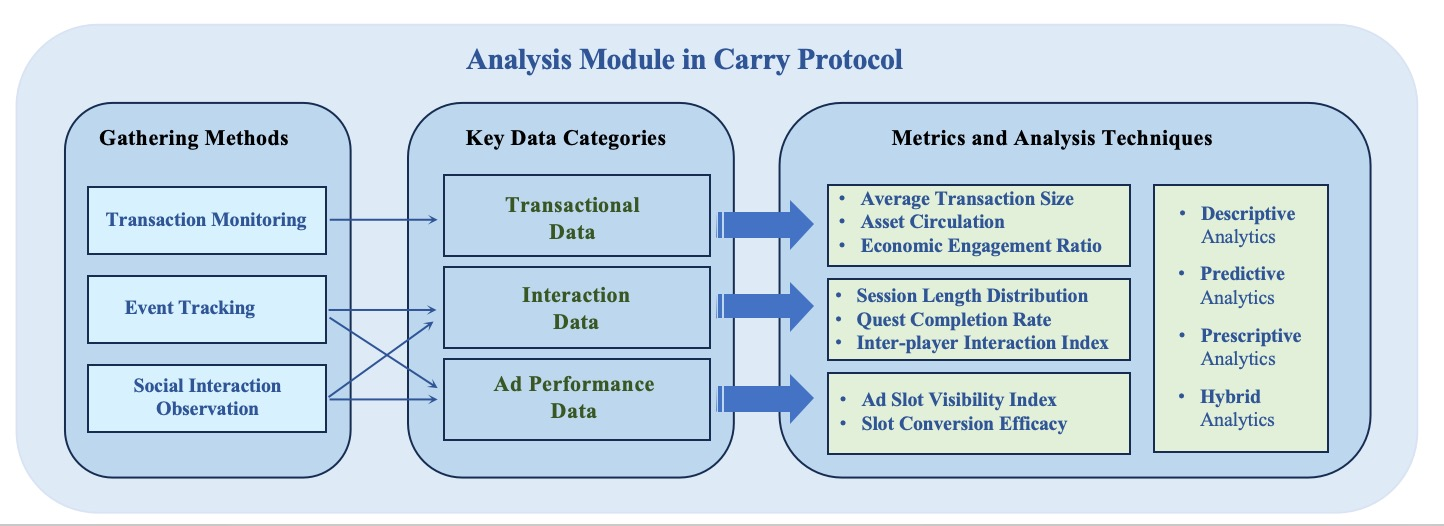
\includegraphics[width=1.0\textwidth]{data analysis.jpg}
    \caption{Data Analysis Framework in Carry Protocol}
    \label{fig:analysis}
\end{figure}



\subsection{Data Types and Metrics}
In this section, we provide detailed data types and significant performance metrics according to the analysis objectives mentioned above.
\subsubsection{Key Data Categories}
For each analytical objective, specific data types are necessary to provide actionable insights.
\begin{enumerate}
    \item \textbf{Transactional Data:} Every in-game transaction, from item purchases to currency exchanges, reflects the game's economic health. Analyzing this data helps in identifying trends, detecting anomalies, and understanding the flow of virtual economies.
\item \textbf{Interaction Data:} Player interactions, both with the game environment and with other players, shed light on community dynamics and engagement levels. This data is invaluable for community management and for enhancing multiplayer aspects of the game.
\item \textbf{Ad Performance Data:} Data on ad views, clicks, and conversions is essential for measuring the effectiveness of in-game advertising. This data category helps advertisers understand the impact of their ads and adjust campaigns for maximum engagement.
\end{enumerate}

\subsubsection{Performance Benchmark Metrics}
% Effective metrics are pivotal for measuring the success of in-game elements and advertising.
% \begin{enumerate}
%     \item \textbf{View Metrics:} These metrics assess how often ads are viewed, offering insights into ad placement and visibility within the game's landscape.
% \item \textbf{Engagement Metrics:} Engagement metrics reveal how players interact with ads, indicating the effectiveness of ad content and design in capturing player attention.
% \item \textbf{Conversion Metrics:}
% Conversion rates measure the success of ads in prompting desired actions, such as in-game purchases or sign-ups, key for evaluating ROI for advertisers.
% \end{enumerate}
Performance Benchmark Metrics within the Carry Protocol are carefully crafted indicators that provide actionable insights derived from specific on-chain data categories. These metrics are designed to evaluate the effectiveness of both the in-game economy and advertising strategies. Here are several refined metrics derived from three aforementioned data types:
\begin{itemize}
    \item \textbf{From Transactional Data:}
    \begin{enumerate}
        \item Average Transaction Size: Indicates the average amount of currency used in transactions, reflecting player spending habits and economic health.
\item Asset Circulation: Measures how frequently in-game assets change hands, revealing the liquidity and dynamism of the game's market.
\item Economic Engagement Ratio: Compares active players to economic transactions, identifying how deeply players are engaged with the in-game economy.
 \end{enumerate}

\item \textbf{From Interaction Data:}
 \begin{enumerate}
     \item Session Length Distribution: Shows the range and average lengths of time players spend in-game per session, indicating engagement depth.
\item Quest Completion Rate: Tracks the percentage of completed in-game quests, measuring content engagement and potential areas for content optimization.
\item Inter-player Interaction Index: Quantifies the interactions between players, such as trades or cooperative play, highlighting the game’s social dynamics.
 \end{enumerate}
\item \textbf{From Ad Performance Data:}
 \begin{enumerate}
\item Player Response Time: Records the time it takes for players to interact with an ad after it appears, indicating the initial impact and relevance of the ad content.
\item Slot Conversion Efficacy: Analyzes the rate at which ad impressions lead to desired player actions, such as in-game purchases or sign-ups, offering a direct measure of ad effectiveness.
 \end{enumerate}
\end{itemize}
The resulting metrics serve distinct purposes.
For Game Developers, they enable fine-tuning of game mechanics to improve player retention, balance the in-game economy, and enhance overall player satisfaction.
For Advertisers, these metrics provide a granular understanding of how different player segments interact with advertisements, informing targeted marketing strategies and creative ad content development. Ultimately, these metrics not only illuminate the current state of game and ad performance but also inform predictions and guide future improvements. They are the linchpin for optimizing GameFi experiences and ensuring that both players and developers reap the maximum benefits from their interactions within the ecosystem.

\subsection{Data Collection and Analysis Techniques}
\subsubsection{Gathering Methods}
The granularity and accuracy of data collection determine the quality of insights derived. 
\begin{itemize}
    \item \textbf{Event Tracking:} This method is leveraged for player interaction data, including player actions, in-game achievements, quest completions, etc. Capturing in-game events provides a detailed picture of player behavior and game mechanics efficacy, allowing for granular analysis and immediate feedback for iterative development. Through an SDK or API integrated into the game client, player operations and game events are captured in real-time. Then, each event is tagged and categorized for deep analysis, such as player progress, preferences, and areas of friction.
\item \textbf{Transaction Monitoring:} This method is leveraged for economic activity data, encompassing player-to-player transactions, purchases of virtual items, currency liquidity, etc. By real-time recording and indexing of all in-game and inter-game transactions using smart contracts and blockchain event logs, Carry Protocol can provide real-time data on economic activities, facilitating a responsive approach to economic management within the game. Finally, it enables developers to monitor and adjust in-game economic policies, prevent inflation, and ensure the health and sustainability of the game economy. Figure~\ref{fig:monitoring} introduced by \href{https://www.wipro.com/blockchain/monitoring-and-management-of-blockchain-networks/}{wipro} represents a blockchain monitoring framework.

\begin{figure}[!htb]
    \centering
    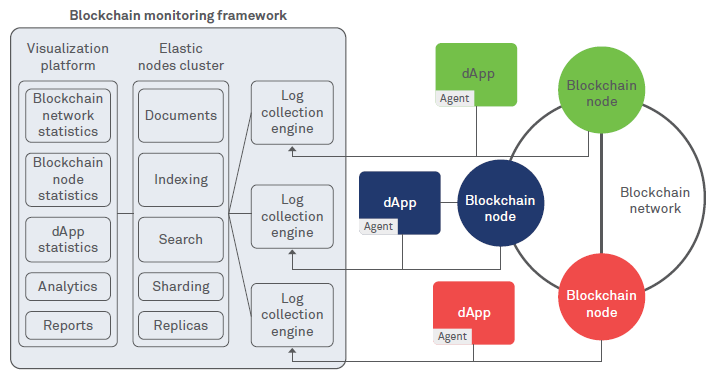
\includegraphics[width=0.9\textwidth]{monitoring-and-management-of-blockchain-networks-2.png}
    \caption{Transaction Monitoring Framework}
    \label{fig:monitoring}
\end{figure}
\item \textbf{Social Interaction Observation:} This method is leveraged for community engagement data, such as communications between players, collaboration, and formation of social networks within the game.
These data collected by analyzing players' in-game chat logs, teamwork, and social interaction events.
Insights into the community's vibrancy, social structure, and player engagement levels can be gleaned from social interaction data. Developers can design more attractive social features and events based on these insights, encouraging interaction and collaboration among players.
\end{itemize}

\subsubsection{Analytical Methodologies}
Each data type requires a specific analysis approach to transform raw data into meaningful insights.
\begin{itemize}
    \item \textbf{Descriptive Analytics:}
This foundational method summarizes raw data into interpretable formats, establishing a baseline understanding of in-game and economic activities. For example, we can aggregating transactional data to compute average transaction size, volume, and frequency over specific time intervals. By analyzing these aggregates, developers can understand the peak times of economic activity within the game, identify spending patterns, and potentially discover underutilized areas of the game economy that could be developed further.
\item \textbf{Predictive Analytics:}
Using statistical models and machine learning algorithms, predictive analytics forecasts future trends, informing proactive game and economic development strategies. For example, we can employ machine learning models, such as decision trees or neural networks, to predict player churn based on interaction data like session length, frequency of play, and engagement in community events. These predictions enable developers to proactively implement features or incentives aimed at retaining players at higher risk of churn, effectively increasing overall engagement and player lifetime value. For example, \href{https://cloud.google.com/blog/topics/developers-practitioners/churn-prediction-game-developers-using-google-analytics-4-ga4-and-bigquery-ml}{Google Cloud} proposed to use BigQuery ML on the sample app dataset to predict propensity to user churn or not churn based on users' demographics and activities within the first 24 hours of app installation.
\begin{figure}[!htb]
    \centering
    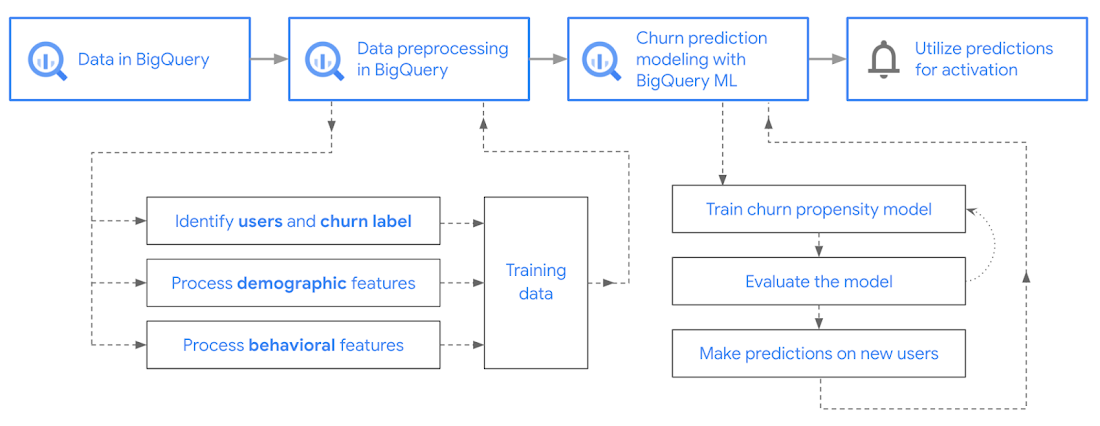
\includegraphics[width=1\textwidth]{prediction.png}
    \caption{Predictive Analytics Framework Proposed by Google Cloud}
    \label{fig:prediction}
\end{figure}
\item \textbf{Prescriptive Analytics:}
Beyond predicting future trends, prescriptive analytics suggests concrete actions to achieve desired outcomes, such as improving user retention or optimizing ad placements. For example, we can utilize advanced analytics, such as optimization algorithms or simulation models, to analyze click-through rates (CTR), conversion rates (CR), and ad exposure duration across different player segments.
Insight: This analysis can suggest which ad content is most effective for specific player demographics or in-game contexts, guiding advertisers on how to tailor their campaigns. For example, if certain ad placements consistently lead to high conversion rates among players who enjoy PvP content, similar strategies can be applied to target this player segment more effectively.
\item \textbf{Combining Methodologies for Comprehensive Insights:} By integrating descriptive, predictive, and prescriptive analytics, Carry Protocol can offer a holistic view of the game's ecosystem. For instance, descriptive analysis of transactional data may reveal an increasing trend in virtual item purchases. Predictive analytics could then forecast this trend's continuation based on current game dynamics and player behavior. Finally, prescriptive analytics could recommend specific in-game events or promotions to capitalize on this trend, such as limited-time offers on popular items or introducing new items likely to be popular based on player preferences inferred from past data.

\end{itemize}

By addressing these objectives, categories, and methodologies, Carry Protocol's data analysis SDK will empower developers and advertisers with the tools needed to unlock the full potential of GameFi. This structured approach ensures that every facet of the gaming experience and economy can be analyzed, optimized, and enhanced for the benefit of all stakeholders in the ecosystem.

\section{General Infrastructure for Both Web2.0 and Web3.0 Games}


At the most basic level, Carry SDK assists developers in integrating blockchain technology into both traditional and emerging Web3 games. It does not mean building every blockchain game from scratch to completion, which takes a massive amount of time and is a non-standardized process that serves only a limited number of users. From the perspective of efficiency, we want this integration to be a standardized and minimized process.
% \begin{figure}[!htb]
%     \centering
%     \includegraphics[width=1.0\textwidth]{gameinfra.png}
%     \caption{Carry Game Infrastructure provides support for both Web2 and Web3 games in multiple aspects.}
%     \label{fig:gameinfra}
% \end{figure}

Specifically, the proposed infrastructure is composed of three fundamental modules (Asset Management Module, Identity Management Module, and Security Protection Module) and two novel modules (Ad Managment Module and Data Analysis Module). 

\subsection{Asset Management Module}
% We will first need to clarify the core differences between traditional and blockchain games to begin this process. In blockchain games, users control their own game assets, independent of any distinguishable facets of gameplay or mechanics. 

% Carry Game Infrastructure is addressing a critical issue in games: the ownership and control of in-game assets. Traditionally, these assets are merely data on a server, which doesn't guarantee players' permanent control over them. Carry uses blockchain concepts, specifically fungible and non-fungible tokens (FTs \& NFTs), to give players a more reliable way to own and use their assets within games. This shift means that the existence and ownership of an asset aren't solely tied to the game itself but are secured on the blockchain.
The Asset Management Module aims to revolutionize the ownership and tradeability of in-game assets through blockchain technology. By leveraging fungible tokens (FTs) for in-game currencies and non-fungible tokens (NFTs) for unique items, this module ensures true ownership, provenance, and interoperability of assets across different gaming platforms and ecosystems. The core designs are composed of the following three elements:
\begin{itemize}
    \item \textbf{Tokenization:} Utilizing ERC-20 (for FTs) and ERC-721 or ERC-1155 (for NFTs) standards to represent in-game currencies and items on the blockchain.
\item \textbf{Smart Contracts:} Deploying smart contracts to handle the logic for asset creation, ownership transfer, and transactions, ensuring transparency and security.
\item \textbf{Blockchain Layer:} Integration with a blockchain layer (e.g., Ethereum, Binance Smart Chain) for decentralized asset management and to leverage its security protocols.
\end{itemize}

Based on the elements mentioned above, the processes can be summarized as follows: 
\begin{enumerate}
    \item Define asset classes and attributes in smart contracts.
    \item Deploy contracts to the blockchain, generating a unique address for each asset.
    \item Implement game logic to interact with blockchain for asset transactions using Carry SDK.
    \item Use event listeners for real-time updates on asset state changes within the game environment.
\end{enumerate}




\subsection{Identity Management Module}
% In the realm of user identity, traditional games rely on conventional methods like email addresses or social accounts for user registration and login. Carry introduces a new paradigm with Web3, where on-chain addresses become the primary identifier. This approach extends the scope of user interaction beyond just games, as the user's identity and activities are independent of the game server. However, integrating these blockchain elements into games has been challenging for many developers, especially those with extensive experience in traditional game development but limited knowledge of blockchain technology.

% To bridge this gap, Carry has developed a comprehensive Software Development Kit (SDK), making it easier for developers to include blockchain features in their games without needing extensive blockchain expertise. The SDK facilitates the binding of a player's wallet address to their game account, allowing a combination of in-game and blockchain-based accounts. It also enables the tokenization of in-game assets, aligning them with corresponding blockchain contracts. This functionality extends to various asset interactions, such as token generation, minting, and transfers, directly through players' Web3 wallets. Carry's SDK, designed for simplicity and security, provides a range of standardized APIs that developers can use to set up a token-based game economy. It supports various blockchain networks and is compatible with multiple client platforms, enhancing its versatility. 
This module seeks to establish a decentralized identity system that allows game players to use a single, secure, and persistent identity across both Web2 and Web3 gaming platforms. By incorporating Decentralized Identifiers (DID) \cite{reed2020decentralized}, it aims to enhance user privacy, security, and cross-platform interoperability. The core designs are composed of the following three elements:
\begin{itemize}
    \item \textbf{DID Integration:} Utilizing the DID standard for creating verifiable, self-sovereign digital identities tied to blockchain addresses.
\item \textbf{Wallet Binding:} Facilitating the binding of a player’s wallet to their game account, enabling seamless in-game and blockchain interactions.
\item \textbf{SDK Features:} Providing APIs within Carry SDK for easy integration of DIDs, supporting login, authentication, and asset management.
\end{itemize}

\begin{figure}[!htb]
    \centering
    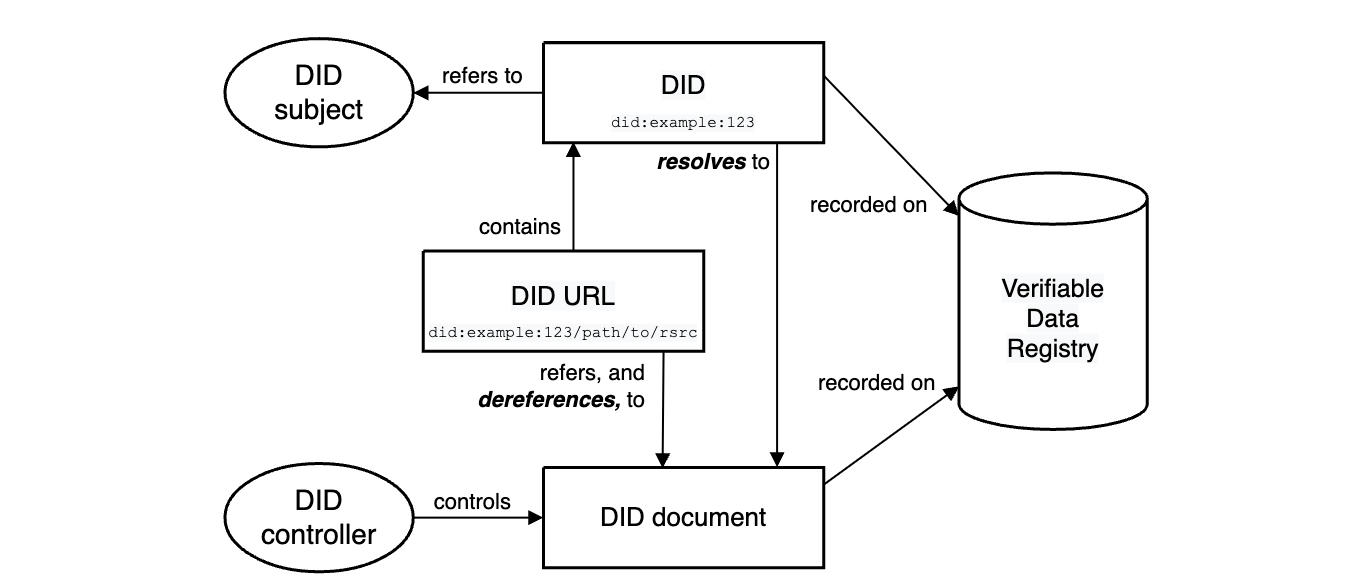
\includegraphics[width=\textwidth]{did.png}
    \caption{Overview of DID architecture and the relationship of the basic components.}
    \label{fig:did}
\end{figure}
We introduce a basic overview of the major components of Decentralized Identifier architecture provided by \href{https://www.w3.org/TR/did-core/}{W3C}, as shown in Figure~\ref{fig:did}. Based on the elements mentioned above, the processes can be summarized as follows: 

\begin{enumerate}
    \item Initialize DID for each user upon registration using Carry SDK.
    \item Bind user's wallet address to their game account, linking in-game and blockchain identities.
    \item Authenticate user actions in-game and on blockchain via digital signatures.
    \item Store and manage user's digital assets and identity securely on-chain.
\end{enumerate}


\subsection{Security Protection Module}
% The SDK also prioritizes security, incorporating features like multi-party computation and private key management mechanisms to ensure the safety of transactions and digital assets within the game environment.
The focus is on ensuring the integrity and security of in-game transactions and digital asset management. By incorporating advanced cryptographic techniques such as multi-party computation (MPC) \cite{feng2023efficient} and zero-knowledge proofs (ZKP) \cite{wang2023zero}, this module aims to protect user assets, maintain privacy, and secure transactions without compromising on user experience.  The core designs are composed of the following three elements:
\begin{itemize}
\item \textbf{Cryptography:} Implementing MPC for secure, distributed private key management and ZKP for transaction validation without revealing sensitive information.
\item \textbf{Smart Contract Security:} Employing security practices like audits and formal verification to ensure smart contract integrity.
\item \textbf{SDK Security:} Ensuring the Carry SDK incorporates the latest security protocols for interaction with blockchain networks, including secure API calls and encryption of sensitive data.
\end{itemize}
 Based on the elements mentioned above, the processes can be summarized as follows: 

\begin{enumerate}
    \item Implement MPC protocols for key management, allowing transactions without exposing private keys.
    \item Use ZKP for transaction validation, ensuring privacy and security.
    \item Conduct regular security audits and update smart contracts and SDK accordingly.
    \item Integrate secure, encrypted communication channels within Carry SDK for asset and identity management.
\end{enumerate}

\subsection{Technical Architecture for Carry SDK}

The above modules collectively provide a robust framework for integrating blockchain technology into gaming, offering a seamless bridge between traditional (Web2) and blockchain-based (Web3) gaming experiences. Through these advancements, Carry Protocol aims to enhance ownership, interoperability, and security for the gaming community. In this section, we demonstrate the detailed technical architecture for Carry SDK, as shown in Figure~\ref{fig:modules}.  

\begin{figure}[!htb]
    \centering
    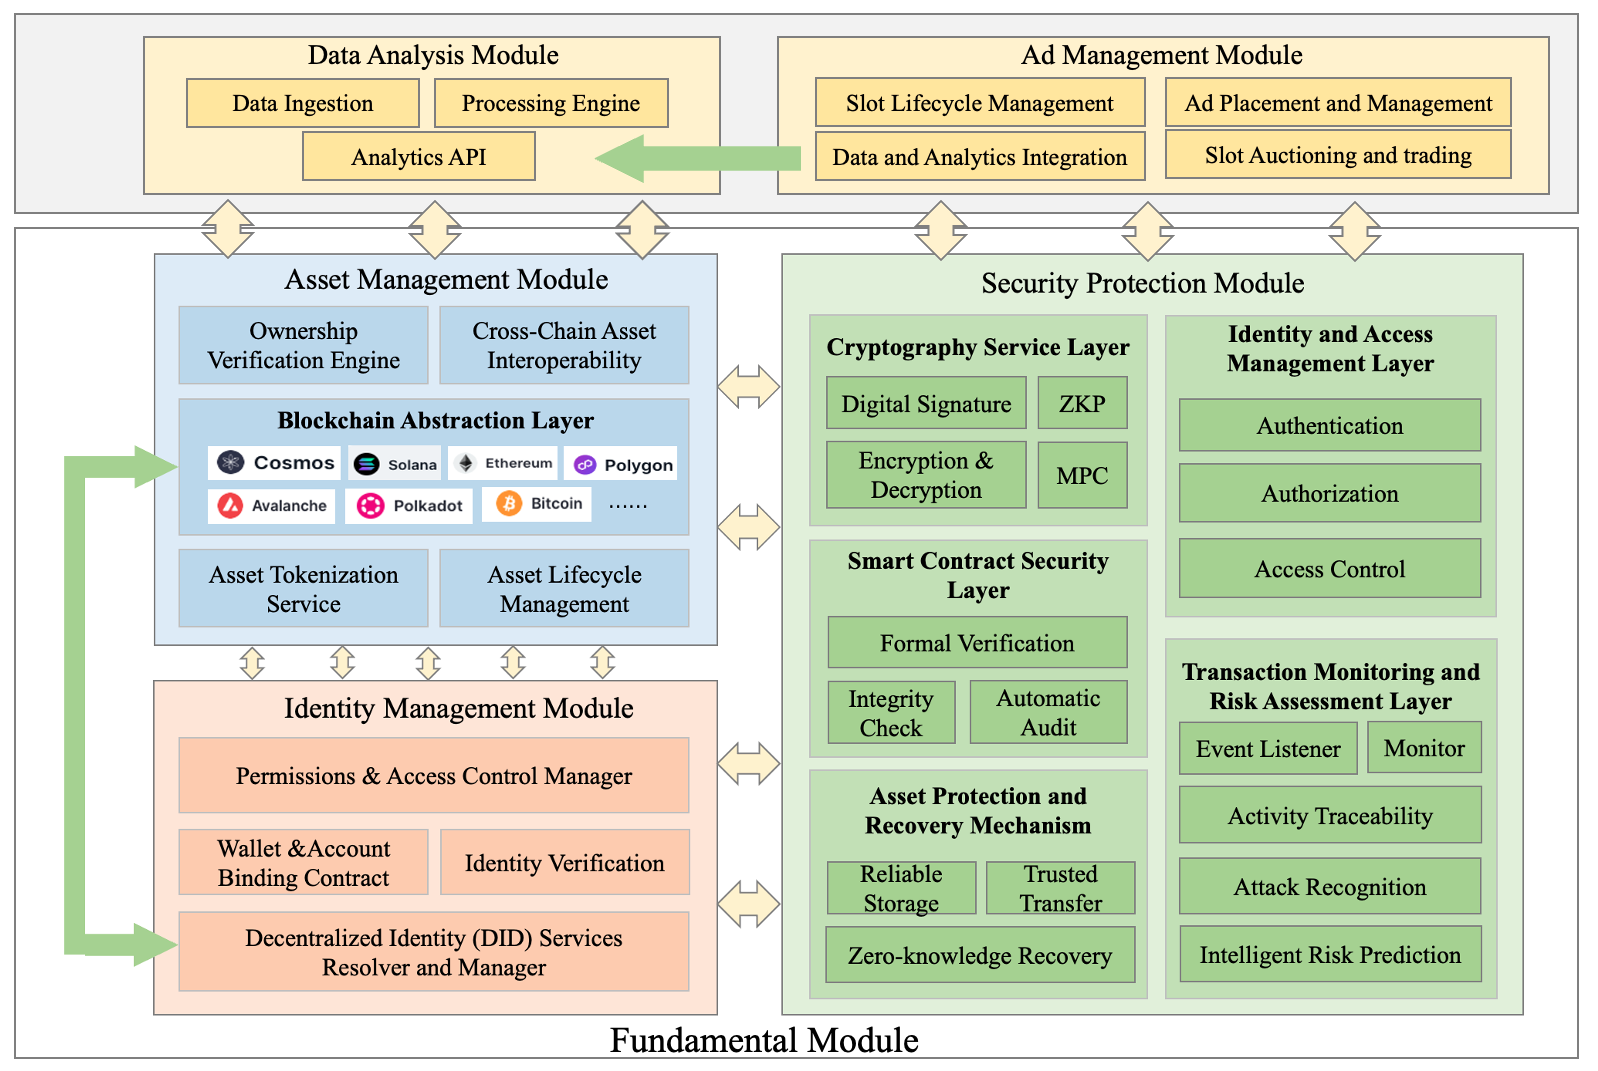
\includegraphics[width=\textwidth]{Technical Architecture Overview of Carry Modules.png}
    \caption{Technical Architecture Overview of Carry SDK Modules.}
    \label{fig:modules}
\end{figure}

\subsubsection{Asset Management Module} 
There are five key components in Asset Management Module. We explain them in a bottom-up manner.
\begin{itemize}
    \item  \textbf{Asset Tokenization Service (ATS):} Converts in-game assets into blockchain tokens. It supports multiple standards (ERC-20, ERC-721, ERC-1155) and manages the lifecycle of tokens including creation, transfer, and destruction.
  \item \textbf{Blockchain Abstraction Layer (BAL):} Serves as the interface between game servers and various blockchain networks, abstracting the complexity of blockchain protocols and offering a unified API for asset transactions.  Interfaces with various blockchains to abstract complexities, providing a unified API for asset transactions across networks like Cosmos, Ethereum, Solona, Polygon, and Binance Smart Chain.
  \item \textbf{Ownership Verification Engine (OVE):} OVE verifies the ownership and authenticity of in-game assets through immutable transactions. This verification process is critical for preventing fraud, duplication, or unauthorized access to assets, thereby ensuring that only rightful owners can initiate transfers or modifications. By providing a trustless mechanism for ownership verification, OVE plays a key role in maintaining a secure and fair gaming environment, where players have full confidence in the value and authenticity of their digital possessions.
  \item \textbf{Cross-Chain Asset Interoperability (CCAI):} Cross-Chain Asset Interoperability (CCAI) addresses one of the key challenges in the blockchain space: enabling assets to move freely and securely across different blockchain networks. CCAI facilitates the trading and exchange of assets between disparate blockchains, enhancing their liquidity and usability. This interoperability is crucial for creating a unified gaming economy where assets from one game or platform can be utilized or traded in another, regardless of the underlying blockchain. By breaking down the barriers between blockchain ecosystems, CCAI enables a more interconnected and fluid digital asset market, where players can leverage the full potential of their in-game assets across the blockchain universe.
\end{itemize}

\subsubsection{Identity Management Module}
There are five key components in Identity Management Module. 
\begin{itemize}
\item \textbf{Decentralized Identity Services:} Decentralized Identity Services form the backbone of the identity management module in Carry Protocol SDK, focusing on managing user identities through decentralized identifiers (DIDs). These services are responsible for the creation, resolution, updating, and revocation of DIDs. By associating a user's DID directly with their game account, it facilitates cross-platform identity verification and usage. DIDs serve as a universal identity marker across different games and platforms, enabling a seamless gaming experience. This system ensures that identities are portable, self-sovereign, and can be verified without reliance on centralized authorities.
\item \textbf{Wallet and Account Binding:} The Wallet and Account Binding component is tasked with securely linking a user's blockchain wallet address to their gaming account. This process is integral for enabling in-game identity verification and asset management through DIDs. By binding the wallet address with the user's DID, it ensures that the user can leverage their blockchain identity within the gaming environment. This linkage is crucial for authenticating transactions and interactions within the game, ensuring that in-game assets and achievements are securely tied to the user's blockchain identity, facilitating a transparent and trustless ecosystem for asset ownership and exchange.
\item \textbf{Identity Verification:} Identity Verification is a critical process within the identity management module that ensures the authenticity of users by leveraging their DIDs. This component utilizes cryptographic methods to verify that actions, transactions, or access requests are genuinely initiated by the rightful owner of the DID. The process involves validating the user's digital signatures and ensuring that the DID associated with a game account matches the blockchain-verified identity. This layer of verification is pivotal for maintaining the integrity of in-game interactions, preventing impersonation, and ensuring that all transactions are securely authenticated.
\item \textbf{Permissions \& Access Control Manager:} The Permissions \& Access Control Manager governs the access rights of users within the gaming environment, based on their DIDs and predefined access policies. This component is essential for defining and enforcing the rules that determine what resources a user can access and what actions they can perform within a game. By leveraging the user's DID for access control, it ensures that only verified and authorized users can interact with sensitive in-game assets or perform certain operations. This mechanism enhances the security of in-game assets and data, preventing unauthorized access and ensuring that game environments remain safe and fair for all participants.
\end{itemize}

\subsubsection{Security Protection Module}
There are five primary components in Security Protection Module. 
\begin{itemize}
    \item \textbf{Cryptography Service Layer (CSL):} The Cryptography Service Layer (CSL) is a foundational component of the security guarantee module, dedicated to providing robust encryption and decryption services. It supports advanced cryptographic technologies, including digital signatures for verifying the integrity and origin of data, as well as Zero-Knowledge Proofs (ZKP) to facilitate transactions and validations without compromising user privacy. By leveraging ZKP and other cryptographic methods, CSL plays a crucial role in ensuring that sensitive user information and transaction details remain confidential, thereby bolstering privacy protection across the blockchain network.
 \item \textbf{Smart Contract Security Framework (SCSF):} The Smart Contract Security Framework (SCSF) focuses on the development and deployment of secure smart contracts, incorporating automated security audits and formal verification processes to identify and rectify common vulnerabilities. This framework ensures that smart contracts, which govern the logic and execution of blockchain transactions, are devoid of loopholes that could lead to unauthorized access or asset theft. By subjecting all smart contracts to rigorous testing and verification, SCSF ensures the integrity of the contracts, safeguarding assets against exploitation and enhancing overall contract security.
 \item \textbf{Identity and Access Management Layer (IAM):} The Identity and Access Management Layer (IAM) manages user identities and access rights, utilizing Decentralized Identity Verification (DID) to enhance security measures. By employing DIDs alongside multi-factor authentication, IAM ensures that only authenticated users can access sensitive operations and data. This approach to identity management not only strengthens security by verifying user identities but also enhances user control over personal information and privacy, ensuring secure and authorized access within the blockchain ecosystem.
 \item \textbf{Transaction Monitoring and Risk Assessment Layer (TMRAS):} The Transaction Monitoring and Risk Assessment Layer (TMRAS) is tasked with the real-time surveillance of blockchain transaction activities. Utilizing machine learning and behavioral analysis techniques, TMRAS assesses the risk levels of transactions, identifying and mitigating potential threats of fraud and theft. This proactive approach to transaction security allows for the timely detection of suspicious activities, ensuring the protection of assets and maintaining the integrity of the blockchain network.
\item \textbf{Asset Protection and Recovery Mechanism (APRM):} The Asset Protection and Recovery Mechanism (APRM) provides a robust defense against unauthorized access and attacks on user assets. Offering solutions for asset recovery in the event of security incidents, APRM ensures the safe storage and transfer of user assets. By implementing measures to quickly restore assets following a breach or loss, APRM plays a critical role in maintaining user trust and confidence in the blockchain's ability to secure digital assets against potential threats and vulnerabilities.
\end{itemize}

\subsubsection{Ad Management Module}
Following the design of core modules in the Carry SDK framework, such as the Asset Management Module, Identity Management Module, and Security Guarantee Module, Carry Protocol introduces a new component: the Ad Management Module. This module is designed to offer an innovative advertising paradigm based on "slots" in blockchain games, integrating advertisements naturally within the game while delivering value to both game developers and advertisers. There are four core components of the Module Framework.
\begin{itemize}
    \item  \textbf{Slot Lifecycle Management:} This component is responsible for overseeing the entire process of a slot's lifecycle, from creation and initialization to the display and updating of advertisements. Game developers can integrate special slots into their games with ease. Once these slots are in place, they can be utilized by developers or players, transforming them into unique digital items. Monitors and updates the status of each slot, ensuring accurate representation within the ecosystem. Intelligently manages the cooperation between different game elements, especially when changes occur.

\item  \textbf{Ad Placement and Management:} Controls the display of advertisement content across various slots, including the addition, removal, and refresh of ads. Once a slot is selected, relevant advertising content is imbued within it. Assesses the impact of displayed advertisements on users or gamers, beginning to generate value.

\item  \textbf{Slot Auctioning and Trading:} Provides a mechanism for the time and positioning of slots to be bid upon and allocated based on market demand and perceived value. Following operations similar to platforms like OpenSea, slots undergo an auction or selection process. Slots are typically leased for a specified duration rather than transferring ownership.

\item  \textbf{Data and Analytics Integration:} Closely integrates with the Data Analysis Module, offering in-depth analysis of ad effectiveness and slot performance. Utilizing the functionalities of the Data Analysis Module, metrics such as click-through rates and conversion rates are analyzed to provide precise advertising strategies for advertisers.
\end{itemize}
By incorporating the Ad Management Module as part of the Carry SDK framework, the Carry Protocol not only redefines the way advertisements are incorporated into video games but also provides new avenues for collaboration between game creators and players. This innovative approach promises to make the gaming experience more engaging while addressing the ownership of digital ad spaces, potentially bringing positive transformations to both the gaming and advertising industries.

\subsubsection{Data Analysis Module}
In addition to the above components, the Data Analysis SDK is structured to seamlessly work within the Carry Protocol ecosystem, enhancing its functionality with dedicated components for comprehensive data analytics. This module is composed of the following three primary components: 
\begin{itemize}
 \item \textbf{Data Ingestion Module:} This component is responsible for capturing both on-chain data and in-game activity data. It employs interfaces that facilitate the streaming of diverse data types into the system, ensuring that data is accurately and efficiently collected for analysis.

 \item \textbf{Processing Engine:} At the core of the SDK is the Processing Engine, which utilizes advanced algorithms for real-time data analysis. This engine processes data from various sources, applying descriptive, predictive, and prescriptive analytics to transform raw data into actionable insights.

 \item \textbf{Analytics API:} The API provides endpoints for accessing the analytics results, allowing developers and advertisers to query specific data points and retrieve insights. This component ensures that the data analysis results are accessible, interpretable, and ready for application.
\end{itemize}


By integrating the Data Analysis Module within the Carry SDK framework, the Carry Protocol ensures that game developers and advertisers have access to a comprehensive suite of tools for data-driven decision-making. This holistic approach not only enhances the gaming experience and economic viability but also enriches the advertisement strategy, making the Carry Protocol a robust foundation for GameFi projects.

\subsubsection{Module Interactions}
% The Carry SDK is meticulously architected to ensure seamless integration and symbiotic relationships among its three core modules: the Identity Management Module, Asset Management Module, and Security Protection Module. At the heart of this integration is the Identity Management Module, which establishes a secure and verifiable framework for user identities using decentralized identifiers (DIDs). This module not only underpins user authentication and access control but also facilitates the secure management and transfer of assets by linking user identities to their digital assets and transactions. The Asset Management Module leverages this secure identity foundation to tokenize in-game assets and manage their lifecycle on the blockchain, ensuring that asset ownership is indisputably tied to the user's identity. This process is further safeguarded by the Security Protection Module, which envelops both the identity and asset management operations in a layer of robust cryptographic services, smart contract integrity checks, and real-time monitoring for transactions and risks. Together, these modules create a comprehensive ecosystem where user identities are securely managed, assets are reliably tokenized and protected, and all interactions within the platform are monitored and secured against potential threats, ensuring a trustworthy and user-centric blockchain gaming experience.
The Carry SDK orchestrates seamless interactions among its five core modules: Identity Management, Asset Management, Security Protection, Ad Management, and Data Analysis. Central to this ecosystem is the Identity Management Module, which authenticates users and links their identities to digital assets and transactions, forming the basis for secure interactions within the SDK. The Asset Management Module utilizes this identity framework to tokenize in-game assets and manage their ownership, ensuring assets are securely linked to users. The Security Protection Module enhances this setup by providing cryptographic security and integrity checks, safeguarding assets and user data against potential threats. Integrating with these foundations, the Ad Management Module leverages user and asset data to place and optimize in-game advertisements, enhancing player experience and advertising value. The Data Analysis Module complements this by analyzing data across modules, offering insights to refine user engagement, asset management, and ad effectiveness.

Together, these modules create a symbiotic environment where secure asset tokenization, personalized advertising, and comprehensive analytics converge to offer a robust and user-centric blockchain gaming experience.



\section{Economics and Incentive Mechanisms}


The Carry token introduces several new features:

\textbf{Governance Vote}: Each Carry token represents a vote in the platform's governance process. The more tokens held in a wallet, the greater the holder's influence and voting power on proposals.

\textbf{Medium of Exchange}: All transactions within the platform can be settled using Carry tokens, with fees and rewards generated during the transaction process distributed in Carry tokens.

\textbf{Collateral}: Carry token holders can use their tokens as collateral to access additional services provided by the platform, including identity management, asset management, security protection, and SDK provision.

\textbf{Membership}: Participants can obtain membership through payment and by providing collateral, which includes access to data analysis, market advice, and additional services such as identity management, asset management, security protection, and SDK provision.

\textbf{Auction Marketplace Creation}: The ad auction process within the Carry ecosystem is vulnerable to several hard-to-prevent attacks, including collusion and witch hunts. Users can use Carry tokens as collateral to create an auction marketplace. The marketplace creator can adjust its parameters, and manage the transaction process, but cannot manipulate the transaction outcomes. The main responsibility of the creator is to regulate participant behavior and to mitigate certain attacks that are currently difficult to prevent against the VCG mechanism. Furthermore, the creator's behavior will be monitored, and abnormal activities will trigger a penalty vote.

\textbf{Carry-Game Token AMM Pool}: The Carry platform will offer services for numerous games. In the future, we will provide a game asset Dex service, allowing users to exchange assets across various games using Carry tokens as an intermediary. Token holders can create an AMM pool for liquidity mining by providing collateral.

\subsection{Governance and Collateral}
Carry aims to be a decentralized service platform for games. Virtually all interactions within the platform, including parameter designs, development direction, auction methods modifications, auction market creation, and various auction mechanism parameters, will be determined through votes by Carry token holders. The voting process is directly proportional to the number of Carry tokens held, granting token holders proportional voting rights and influence over proposals.

Users can provide Carry tokens as collateral to gain more rights. Basic collateral rights include access to additional services provided by the platform's three modules (identity management, asset management, and security protection), contributions from SDK users in the ecosystem, and penalties for misconduct. Moreover, users can collateralize their assets to earn revenue by creating and managing an auction marketplace. In the future, after establishing the game asset exchange pool, users can also provide liquidity to the exchange pool to earn mining rewards.

\subsection{Customized Auction Market}
The auction process in the Carry ecosystem is susceptible to several hard-to-defend attacks, including collusion and witch hunts. Users can collateralize Carry tokens to establish an auction marketplace, where the creator can adjust its parameters and oversee the transaction process without influencing the outcomes. The creator's primary role is to regulate participant behavior to mitigate certain VCG mechanism attacks that are currently indefensible. The creator's actions will be under surveillance, and any detected abnormal behavior will prompt a penalty vote. Auction marketplace creators could be individual game operators selling in-game ad space or ad space traders managing their traffic. All Carry token holders are eligible to create an auction marketplace, provided they collateralize sufficient Carry tokens and abstain from malicious practices.
% Carry token has even more new features:

% \textbf{Governance Vote}: each Carry token represents a vote in the platform's governance process. The more tokens held in the wallet, the more votes and influence the holder has on proposals.

% \textbf{Medium of Exchange}: All transactions within the platform can be settled in the form of \$Carry tokens, and the fees and rewards generated during the transaction process are distributed by \$Carry tokens.

% \textbf{Collateral:} \$Carry holders can Collateral tokens to use the additional services provided by the platform, including identity management, asset management and security protection, and SDK provision.

% \textbf{Membership}: Participants can obtain membership through payment and Collateral, which includes data analysis, market advice, and additional services such as identity management, asset management and security protection, and SDK provision, etc.

% \textbf{Auction Marketplace Creation}: The ad auction process in the Carry ecosystem is subject to a number of hard-to-prevent attacks, including collusion attacks and witch hunts, among others. Users can Collateral \$Carry to create an auction market. The parameters of the auction market can be adjusted by the creator, and the transaction process in the market will also be managed by the creator, but the creator cannot manipulate the transaction results, and the creator's main job is to control the behavior of the participants, and to prevent some of the currently unpreventable attacks against VCG. Moreover, the creator's behavior will also be monitored, and if abnormal behavior is found, a penalty vote will be initiated.

% \textbf{Carry-Game Token AMM Pool: }Carry platform will provide services for a large number of games, in the future we will provide game asset Dex services, by \$Carry tokens as an intermediary, users can exchange assets in all kinds of games, the Collaterale can create an AMM pool for liquidity mining.

% \subsection{Governance and Collateral}
% Carry will be a decentralized service platform for games. Almost all interactions and parameter designs within the platform, as well as the direction of development, will be voted on by the \$Carry token holders, including the increase or decrease of auction methods, the creation of the auction market, the parameter designs of various auction mechanisms, the future development of the Carry platform, etc. The voting process is positively related to the number of \$Carry tokens held by the token holders. The voting process of the platform's governance is positively correlated with the number of \$Carry tokens held by the token holders, the more \$Carry tokens, the more the holders have the right to vote and influence on the proposal.

% Users can Collateral \$Carry to gain more equity. The equity from the basic Collateral mainly includes additional services provided by the three modules of the platform (identity management, asset management and security protection), contributions from SDK users in the eco-system, and fines for misbehavior, etc., and the Collaterale can participate in the distribution of the revenue. In addition, users can also Collateral their own assets and gain revenue by creating and managing an auction market, and in the future, after the construction of the game asset exchange pool is completed, users can provide liquidity for the exchange pool to gain mining revenue.

% \subsection{Customized Auction Market}
% The auction process in the Carry ecosystem is subject to a number of attacks that are difficult to prevent, including collusion attacks and witch attacks. Users can Collateral \$Carry to create an auction market, the parameters of the auction market can be adjusted by the creator, and the transaction process in the market will also be managed by the creator, but the creator can not manipulate the transaction results, the creator's main job is to control the behavior of the participants, to prevent some of the currently unpreventable attacks against the VCG. Moreover, the creator's behavior will be monitored, and a penalty vote will be initiated when abnormal behavior is detected. Auction marketplace creators can be individual game operators selling in-game ad space, or ad space traders maintaining their own traffic, and all \$Carry token holders can create an auction marketplace, as long as they Collateral enough \$Carry tokens and don't engage in malicious behavior.

\subsection{Auction Mechanisms}
Carry platform provides personalized advertising auction marketplace creation form, so we provide all kinds of mainstream auction mechanism services, including open incremental auction (British auction), open decremental auction (Dutch auction), GFP auctions, GSP auctions, VCG auctions, etc., and additional design of the Dutch auction mechanism and VCG auction mechanism.

\subsubsection{Incremental auction (English auction)}
An Incremental Auction is a type of auction where participants openly bid against each other, with bids increasing in value until no higher bids are offered. This is in contrast to sealed-bid auctions, where bids are submitted privately.

In an Incremental Auction:

1. Open Bidding: The auctioneer starts the bidding process at a certain price, often the minimum acceptable bid. Participants then openly raise the bid in increments, announcing their bids aloud or indicating them through gestures or signals.

2. Incremental Bidding: Bids must exceed the current highest bid by a predefined increment. The auctioneer may announce these increments, and participants must adhere to them when raising their bids.

3. Competitive Bidding: Bidders continue to raise the price until no one is willing to offer a higher bid. This competitive process typically results in the highest possible price for the item being auctioned.

4. Winner Determination: The participant who offers the highest bid when no further bids are made wins the auction and is obligated to pay the final bid amount.

5. Transparency and Participation: Incremental auctions offer transparency as all participants can see each other's bids in real-time, allowing them to make informed decisions about whether to continue bidding.

Incremental auctions are commonly used for selling various types of goods, including antiques, artwork, real estate, and other high-value items. They are also employed in online platforms and platforms for advertising space, where bids are placed electronically and in real-time. The open nature of incremental auctions promotes competition among bidders, often leading to higher prices compared to other auction formats.


\subsubsection{Dutch Auction (Open Descending Price Auction)}
In a Dutch Auction, the price of the ad slot starts high and decreases over time until an advertiser places a bid or the price drops to a reserve price.

\paragraph{Agency Strategy for Dutch Auction:} 
The agency aims to secure the ad slot for its client at the lowest possible price but also needs to balance the risk of losing the slot to another bidder. The strategy could be defined as follows:

\[
B_i(t) = 
\begin{cases} 
0 & \text{if } P(t) > V_i \\
V_i & \text{if } P(t) \leq V_i \text{ and } \text{Risk}(t, V_i) > \theta \\
0 & \text{otherwise}
\end{cases}
\]

Here:
\begin{itemize}
    \item \( B_i(t) \) is the bid from agency \( i \) at time \( t \)
    \item \( P(t) \) is the current price at time \( t \)
    \item \( V_i \) is the agency’s valuation for the ad slot
    \item \( \text{Risk}(t, V_i) \) is a function evaluating the risk of losing the slot if waiting any longer, considering the current time and valuation
    \item \( \theta \) is a risk threshold, beyond which the agency decides to bid to avoid losing the slot
\end{itemize}

In a more sophisticated approach, the agency not only considers the current price and its own valuation but also takes into account the time decay, estimated competition, and a dynamic risk assessment.

\[
B_i(t) = 
\begin{cases} 
0 & \text{if } P(t) > V_i \\
V_i \cdot \left(1 - e^{-\lambda \cdot (T-t)}\right) & \text{if } P(t) \leq V_i \cdot \left(1 - e^{-\lambda \cdot (T-t)}\right) \text{ and } \text{Competition}(t, P(t)) \leq \gamma \\
0 & \text{otherwise}
\end{cases}
\]

Here:
\begin{itemize}
    \item \( T \) is the total time duration of the auction
    \item \( \lambda \) is a parameter controlling the time sensitivity of the bid
    \item \( \text{Competition}(t, P(t)) \) is a function estimating the level of competition based on the current time and price
    \item \( \gamma \) is a competition threshold, beyond which the agency decides not to bid due to high competition
\end{itemize}

In this strategy, the agency increases its willingness to bid as the auction progresses, adjusting its bid according to the time decay function. The agency also evaluates the level of competition at the current price and decides to bid only if the estimated competition is below a certain threshold.

\paragraph{Risk Function and Competition Function Design}

To address the dynamic and complex nature of bidding in a Dutch auction, where the price of an ad slot decreases over time, we propose sophisticated models for evaluating the risk of losing the slot and estimating the level of competition, i.e., $Risk(t, V_i)$ and $Competition(t, P(t))$.



The risk of losing the ad slot increases as the auction progresses and as the current price approaches the agency's valuation of the slot. We model this risk as a function of time and the difference between the valuation and the current price, incorporating market competition. It is calculated as:

\begin{equation}
Risk(t, V_i) = \frac{1}{1 + e^{-\kappa \cdot (V_i - P(t)) \cdot \omega(t)}}
\end{equation}

where:
\begin{itemize}
    \item \( \kappa \) controls the steepness of the function, reflecting how valuation differences affect risk perception.
    \item \( \omega(t) \) is a weight function that increases with time, indicating the growing risk as the auction nears its end. The calculation formula is shown in Equation (4). 
\end{itemize}

\begin{equation}
\omega(t) = \frac{T - t}{T}
\end{equation}


Competition dynamically changes based on multiple factors including the current price, time elapsed, and historical bidding behavior. As the price decreases, the auction may attract more bidders, affecting the competition level. The calculation formula is defined as:

\begin{equation}
\begin{aligned}
Competition(t, P(t)) &= \beta \cdot \log\left(\frac{P(0)}{P(t)}\right) + \eta \cdot \frac{t}{T} \\
&= \beta_0 \cdot \left(1 + \mu \cdot \frac{dP}{dt}\right) \cdot \log\left(\frac{P(0)}{P(t)}\right) + \eta \cdot \frac{t}{T} \\
\end{aligned}
\end{equation}

where:
\begin{itemize}
    \item \( P(0) \) represents the initial price of the ad slot at the start of the auction.
    \item \( \beta \) represents the effect of price decrease on attracting more competition. It can be modeled as a function related to the rate of price decrease, enhancing our understanding of how price dynamics influence competition levels during the auction.
    \begin{equation}
\beta = \beta_0 \cdot \left(1 + \mu \cdot \frac{dP}{dt}\right)
\end{equation}

where:
\begin{itemize}
    \item \( \beta_0 \) is the base competition attractiveness coefficient, indicating the level of competition without price changes.
    \item \( \mu \) is a modulation coefficient that reflects the sensitivity of competition attractiveness to the rate of price decrease.
    \item \( \frac{dP}{dt} \) represents the rate of price decrease, indicating the change in price over unit time.
\end{itemize}

    \item \( \eta \) captures the impact of time on competition, reflecting how urgency among bidders may increase as the auction progresses.
\end{itemize}

These models provide a more accurate representation of the strategic considerations in a Dutch auction, allowing agencies to make informed decisions based on the evolving risk and competition levels.


\paragraph{ROI of Agencies' Strategy}

In a Dutch Auction, the price of the advertising slot decreases over time, and agencies aim to secure slots at an optimal price point that balances cost and potential returns. An advanced bidding strategy should therefore consider both the cost of the slot and the expected return on investment (ROI).

The bid function \( B_i(t) \) for agency \( i \) at time \( t \) can be formulated as:

\[
B_i(t) = 
\begin{cases} 
0 & \text{if } P(t) > V_i \text{ or } \text{ROI}_i(t, P(t)) < \text{ROI}_{\text{threshold}} \\
P(t) & \text{if } P(t) \leq V_i \text{ and } \text{ROI}_i(t, P(t)) \geq \text{ROI}_{\text{threshold}} \text{ and } \text{Competition}(t, P(t)) \leq \gamma \\
0 & \text{otherwise}
\end{cases}
\]

Here:
\begin{itemize}
    \item \( \text{ROI}_i(t, P(t)) \) is the expected return on investment for agency \( i \) at time \( t \) given the current price
    \item \( \text{ROI}_{\text{threshold}} \) is the minimum acceptable ROI for the agency
    \item \( \text{Competition}(t, P(t)) \) is a function estimating the level of competition based on the current time and price
    \item \( \gamma \) is a competition threshold, beyond which the agency decides not to bid due to high competition
\end{itemize}

The function \( \text{ROI}_i(t, P(t)) \) can be further defined based on the agency’s estimation of the ad slot’s effectiveness, the target audience's size, and other relevant factors.  On the basis, ROI can be understood as:

\begin{equation*}
    ROI = \frac{Income}{Spending}
\end{equation*}

In real life the estimation of the real ROI might be more complicated than this. If an agency is conducting one advertisement campaign in one month time, the return can be of the following notation:

\begin{equation*}
        ROI = \frac{\Sigma_i(I_i \cdot N_i - E_i) - \Sigma{C_{slot}}}{\Sigma{C_{slot}}}
\end{equation*}

where:
\begin{itemize}
    \item \( \text{I}_i \) is the item price for \(i\) that has been sold in this campaign duration. 
    \item \( \text{E}_i \) is the expected sales amount of product \(i\).
    \item \( \text{C}_{slot} \) is the cost of a slot.
\end{itemize}


The theoretical returns are a benchmark for the success of any agencies that is on Carry protocol. Real strategy returns can be monitored and calculated through several methods. The Carry measurement and metrics can be used for capturing the real ROIs of any efforts put on the network. Furthermore, we can adopt the P value in the statistics of the sales side to estimate the general impact of certain advertisement campaign.\\

There are metrics that can also be taken into consideration which agencies could measure when trying to estimate the expected outcome for certain collection of slots:

\begin{itemize}
    \item \textbf{Total Crypto Assets of the Slot Owner's Address:} This reflects the financial strength of the slot owner. Agencies can use this information to assess whether the slot owner has enough resources and motivation to maintain and promote their slots, indirectly affecting the advertisement’s effectiveness.
    \item \textbf{Fair Market Price of the Attached NFT to the Slot} This indicates the value of the NFT attached to the slot. High-value NFTs may attract more user attention, potentially increasing the advertisement’s exposure and effectiveness. Agencies can use this information to select slots with high-value NFTs for ad placements.
    \item \textbf{Active User Count of the Onchain Game Associated with the Slot:} This reflects the game’s activity level and user base size. A higher number of active users means more opportunities for ad exposure. Agencies can prioritize games with a large active user base for their ad placements.
\end{itemize}

In addition to the above metrics, agencies can choose from a wider range of dimensions available through the Open Carry Advertisement Network, such as user geographic locations, interests, consumption habits, and more. This allows agencies to offer more precise and personalized ad placement services to advertisers, improving the advertisement’s conversion rate and ROI.

By considering a comprehensive set of relevant metrics, agencies can more accurately estimate advertisement effectiveness, providing more valuable and competitive services to advertisers.

\subsubsection{Generalized first-price auction}
In a GFP auction(Generalized First Price), advertisers bid based on their valuation of the ad space. The advertiser with the highest bid wins the spot and pays the bid they submitted. This auction mechanism is similar to a traditional first price auction, but GFP allows bidders to submit a variety of unconventional bids, such as maximum bids, click-through rates, conversion rates, etc.

The hallmark of a GFP auction is that it promotes competition by allowing bidders to submit their true valuation of the ad space, thus ensuring that the ad space is allocated to the most valuable advertiser. However, despite the advantages of simplicity and guaranteed revenue, GFP auctions are less stable. This is because individual advertisers may modify their placement prices frequently in order to obtain optimal revenue. For example, an advertiser may continually increase its price in order to gain display; after gaining display, it may begin to continually decrease its price in order to reduce costs. This competition is relatively arbitrary and it is easy to know competitors' bids.

In addition, when the advertiser with the highest bid stops placing, it is prone to large fluctuations in ad platform revenue. This is because other advertisers may have lower bids, resulting in a drop in ad platform revenue. Therefore, when using GFP auctions, advertising platforms need to consider how to balance the competition from advertisers and maintain a smooth revenue.


\subsubsection{Generalized Second-Price auction}
In a GSP auction, advertisers bid based on their valuation of the spot, and the highest bidder wins the spot and pays the price offered by the second highest ranked advertiser.

\subsubsection{Vickrey–Clarke–Groves auction}
VCG Auctions are sealed bid auctions of multiple items. Bidders submit bids that report the valuation of their items without knowing the bids of other bidders. The auction system allocates items in a socially optimal manner: it charges each individual for the losses they inflict on other bidders. It incentivizes bidders to bid their true expectations by ensuring that each bidder's best strategy is to bid the true valuation of the item.

The first step in the VCG mechanism is for participants to submit their preferences for resources or items. This may include valuation of different resources, order of preference, or other relevant information. We analyze data from the Carry system to obtain relevant data about the published Slot (including TVL of the game, number of viewers, number of clicks in the past, average revenue in the past, etc.) to calculate the evaluation price of the Slot as the reference price of the Slot. This reference price affects the valuation of the advertiser participants. Based on the participants' preferences and bids, the impact of each possible resource allocation scheme on the overall social welfare is calculated. The social welfare can be expressed in the form of a weighted sum where the utility of each participant is weighted by its weights.

The allocation scheme that maximizes the impact on overall social welfare is chosen as the final resource allocation outcome. Typically, this process involves evaluating all possible allocation options to determine which one is most favorable to overall social welfare. For each participant, the marginal contribution to overall social welfare is calculated, i.e., the amount by which overall social welfare would change if the participant did not participate. This is referred to as the VCG payment.The calculation of the VCG payment usually entails calculating the amount by which overall social welfare would change if the participant were to withdraw.

For any set of auctioned items \( M = \{t_1,\ldots,t_m\} \) and any set of bidders \( N = \{b_1,\ldots,b_n\} \), let \( V^M_N \) be the social value of the VCG auction for a given bid-combination. That is, how much each person values the items they've just won, added up across everyone. The value of the item is zero if they do not win. For a bidder \( b_i \) and item \( t_j \), let the bidder's bid for the item be \( v_{i}(t_{j}) \). The notation \( A \setminus B \) means the set of elements of A which are not elements of B.

A bidder \( b_i \) whose bid for an item \( t_j \) is an overbid, namely \( v_{i}(t_{j}) \), wins the item, but pays \( V^{M}_{N \setminus \{b_i\}}-V^{M \setminus \{t_j\}}_{N \setminus \{b_i\}} \), which is the social cost of their winning that is incurred by the rest of the agents.

Indeed, the set of bidders other than \( b_i \) is \( N \setminus \{b_i\} \). When item \( t_j \) is available, they could attain welfare \( V^{M}_{N \setminus \{b_i\}} \). The winning of the item by \( b_i \) reduces the set of available items to \( M \setminus \{t_j\} \), so the attainable welfare is now \( V^{M \setminus \{t_j\}}_{N \setminus \{b_i\}} \). The difference between the two levels of welfare is therefore the loss in attainable welfare suffered by the rest of the bidders, as predicted, given the winner \( b_i \) got the item \( t_j \). This quantity depends on the offers of the rest of the agents and is unknown to agent \( b_i \).

The winning bidder whose bid is the true value \( A \) for the item \( t_j \), \( v_{i}(t_{j})=A \), derives maximum utility \[ A - \left(V^{M}_{N \setminus \{b_i\}}-V^{M \setminus \{t_j\}}_{N \setminus \{b_i\}}\right) .\]

Additional, hesitation VCG mechanism calculation process is too complicated, we refer to Facebook's VCG mechanism. the Slot reference price of VCG mechanism will be related to CPM (Cost Per Mille) and CTR (Click-Through Rate). Because advertisers' revenue is impossible to know, eCPM is used as an alternative to CPM. eCPM is commonly used to measure the effectiveness of advertisements in an ad network, and it calculates the average revenue generated by an advertisement per 1,000 displays, regardless of whether or not the advertisement is clicked. The eCPM is calculated by dividing the ad revenue by the number of times the ad is displayed and multiplying by 1000. eCPM is given by the formula:

\[ eCPM = \frac{Total\ Revenue}{Impressions} \times 1000 \]

Where Total Revenue represents the total revenue of the advertisement and Impressions represents the number of times the advertisement is displayed. Then calculate
\begin{equation} 
\begin{split}
    CPM \ Paid = Next \ Highest \ Slot \ Bid *(Slot \ eCPM - \ Following \ Slot \ eCPM) \\ 
+ Following \ Slot \ Bid *(Following \ Slot \ eCPM - Subsequent \ Slot \ eCPM).
\end{split}
\end{equation}

The calculation method of deduction, if we strictly follow th e definition of VCG, we need to calculate the revenue loss of all other advertisers all over again, this is a two-tier FOR loop on the line, when there is a lot of depth of ads, this calculation is costly, we only take the 2nd ads under the first price of the first ad position to calculate this loss.



% \subsection{Carry Token Utilization Scenarios}

% \begin{table}[!htb]
%     \centering
%     \begin{tabular}{c|c|c}
%         \toprule
%         Scenatio & Type & Add Value \\
%         \midrule
%         \rule{0pt}{2ex} 
%         Slot placement durations auction & Token &Transaction fees discount  \\
%         \rule{0pt}{2ex} 
%         Ad Content Placement & GAS &  \\
%         \rule{0pt}{2ex} 
%         Slot Initialization &GAS& \\
%         \rule{0pt}{2ex} 
%         Effect tracking & Token & \\
%         \rule{0pt}{2ex} 
%         Slot settlement  & Token & \\
%         \rule{0pt}{2ex} 
%         Issue a Proposal & Governance & \\
%         \rule{0pt}{2ex} 
%         Vote on snapshot & Governance & \\
%         %... add more rows as necessary
%         \bottomrule
%     \end{tabular}
%     \caption{Carry Token Utilizations}
%     \label{table:example}
% \end{table}



% \subsubsection{Users}
% In the traditional advertising ecosystem, users are often the most overlooked participants. Advertising platforms typically assume that since users are already enjoying some basic internet services for free, they should be willing to provide their data and privacy, along with tolerating advertisements. In reality, the commercial value generated from user data has long contributed to the prosperity of the advertising ecosystem. Users, as they engage in internet activities, are not just consumers of services; they actively contribute their data, thereby supporting the ecosystem.\\

% The Carry Protocol believes that users have the right to access the commercial value generated by their data and the ability to choose how their data is utilized. Within the slot framework, the contributions of players and users' data can be transparently tracked, allowing developers, users, and advertisers to negotiate ad settlement terms based on the value of user data.\\

% We encourage developers and advertisers to share a larger portion of the revenue with players and users. This not only increases user engagement but also helps advertisers build more direct relationships with users and foster more adhesive communities, ultimately granting advertisers greater influence over users.


% \subsection{Comparison of Incentive Distribution}

% \begin{table}[!htb]
%     \centering
%     \begin{tabular}{>{\raggedright\arraybackslash}p{2.5cm} p{6cm} p{6cm}}
%         \toprule
%         \textbf{Role} & \textbf{Traditional Ad Platform} & \textbf{Carry Protocol}  \\
%         \midrule
%         \multirow{2}{2.5cm}{Developers} 
%         & Income is limited by platform fees, hindering innovation. 
%         & Direct collaboration with advertisers through slots, increased income, reduced costs.  \\
%         \cmidrule{2-3}
%         & Lack of transparent ad performance data, unfavorable negotiations. 
%         & Access to ad performance data at any time, direct settlement with advertisers. \\
%         \midrule
%         \multirow{2}{2.5cm}{Advertisers} 
%         & High platform fees, opaque data mechanisms lower ROI. 
%         & Directly allocate budgets to developer services, improving ROI and industry efficiency. \\
%         \cmidrule{2-3}
%         & High cost of ad performance testing, data constrained by platforms. 
%         & Use Carry Protocol's measurement metrics for ad performance testing, reducing cost. \\
%         \midrule
%         \multirow{2}{2.5cm}{Users} 
%         & Data and privacy are viewed and contributions with limited benefits. 
%         & Have the right to receive the commercial value of their data, choose whether data is used. \\
%         \cmidrule{2-3}
%         & Participate in internet activities with contributions but no benefits. 
%         & Share more revenue, build more direct relationships and sticky communities.\\
%         \midrule
%         Agencies 
%         & Difficulty in data acquisition limits effectiveness measurement, audience profiling, and campaign optimization. 
%         & Provide more services in Carry Protocol's open advertising ecosystem, improving efficiency.\\
%         \bottomrule
%     \end{tabular}
%     \caption{Comparison of Incentives}
%     \label{table:comparison}
% \end{table}

\section{Protocol Implementation}

\subsection{Carry Slot Contract}

Carry Protocol manages game advertisements through slots. The protocol itself serves as the smart contract which manages the lifecycle of advertisement contents and slots.
\begin{figure}[!htb]
    \centering
    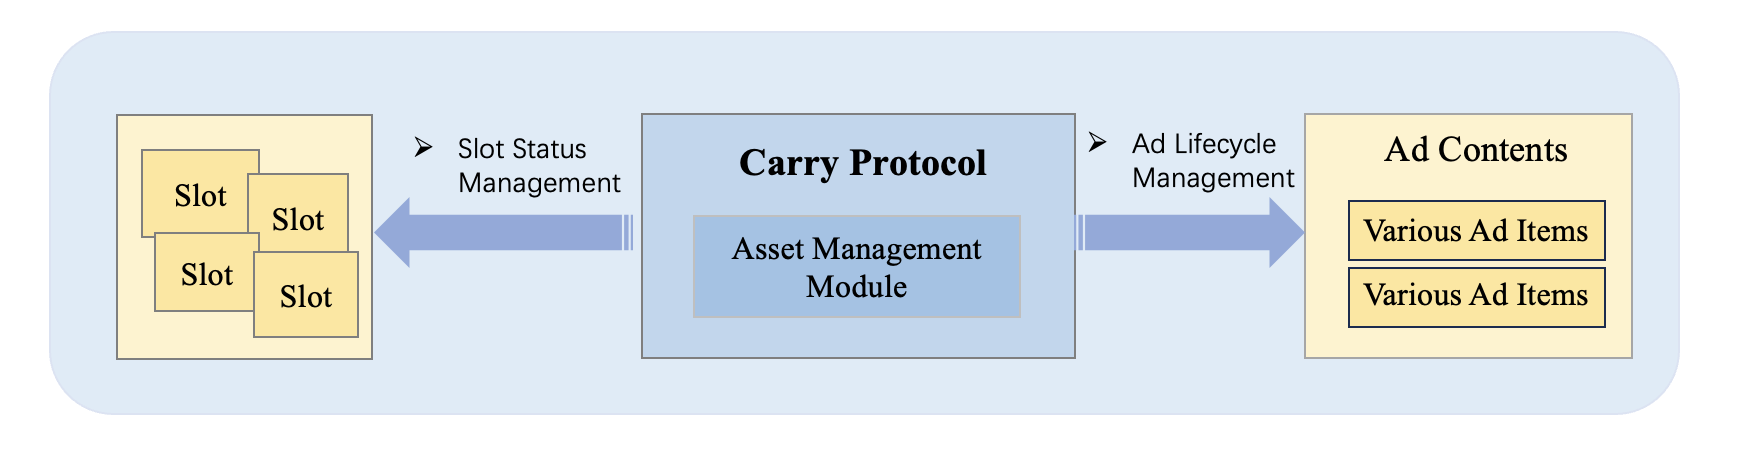
\includegraphics[width=0.9\textwidth]{slotexplain.png}
    \caption{Slot is the basic instrument for Carry Protocol to manage advertisement.}
    \label{fig:slotexplain}
\end{figure}

\subsubsection{Slot Creation}

When a new ad campaign is about to start in a web3 game, the first step is setting up a special ad spot, known as a "slot." This slot is made into a unique digital item, like a one-of-a-kind collectible, which means it's owned and can be traded. Game makers weave these slots into their games, and then either they or the players can activate them, turning them into owned digital assets. It's similar to creating a brand-new collectible item that's ready to be paired with an ad.

\subsubsection{Slot Release}

A slot, once used, may need to be released or made available for future advertisements. This involves the termination or expiration of its current content, making the slot a blank canvas once more. While this could technically be a part of the slot contract, the process's simplicity might not necessitate a full-fledged contract on its own. Instead, it could be an operation under the broader slot management system.


\subsubsection{Slot Content Change}

Over time, advertisements or the content within a slot might need updating or altering. This could be due to changing marketing strategies, game narratives, or even player preferences. The Carry Slot Contract allows for dynamic content modifications, ensuring that the slot remains relevant and engaging. However, it is challenging to alter the embedded contents since slots are mined as valuable assets which are recorded onto blockchain, which exhibits extreme immutability. Therefore, we need to trade off between modifiability and immutability in Carry \cite{ye2023survey}. To this end, we introduce Chameleon Hash algorithm to achieve a redactable transaction property for Carry. The structure is illustrated in Figure\ref{fig:chameleon}~\cite{wu2021quantum}.

\begin{figure*}[!htb]
    \centering
    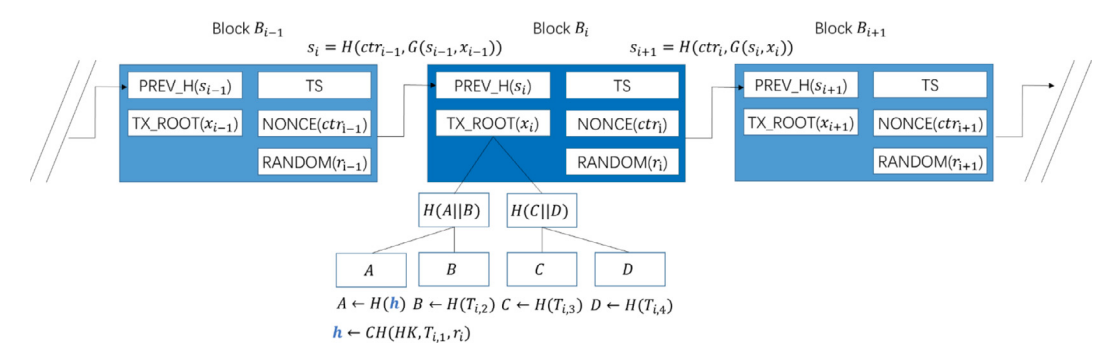
\includegraphics[width=\textwidth]{chameleon hash.png}
    \caption{Chameleon Hash-based Alterable Slot Contents Solution.}
    \label{fig:chameleon}
\end{figure*}

\begin{enumerate}[label=(\arabic*)]
    \item \textbf{Bilinear Pairing.} Let $\mathbb{GF}(p)$ denote a finite field, where $p$ is a large prime number. We consider an elliptic curve $E_p(a,b)$ over $\mathbb{GF}(p)$, which can be defined as the set of ordered pairs $(x,y) \in \mathbb{GF}(p) \times \mathbb{GF}(p)$ that fulfill the condition $y^2 \equiv x^3 + ax + b \;(\text{mod}\; p)$, given that $a, b \in \mathbb{GF}(p)$ and $4a^3 + 27b^2 \not\equiv 0\; (\text{mod}\; p)$. This leads to the construction of an additive cyclic group, denoted $\mathbb{G}_1$, and a multiplicative cyclic group, $\mathbb{G}_2$, both of which have the prime order $p$. These groups are constituted of all points residing on the elliptic curve, complemented by the point at infinity. A random generator of $\mathbb{G}_1$ is designated as $P$. We define a bilinear map $e: \mathbb{G}_1 \times \mathbb{G}_1 \rightarrow \mathbb{G}_2$ (known as a type-1 pairing) that adheres to the following three properties \cite{bagga2023bilinear}:
\begin{itemize}
    \item \textbf{Bilinearity:} For any $X, Y \in \mathbb{G}_1$ and any $a, b \in \mathbb{Z}_p^\ast$, it holds that $e(aX, bY) = e(X, Y)^{ab}$.

\item \textbf{Non-degeneracy:} If we designate $1_{\mathbb{G}_2}$ as the identity element of $\mathbb{G}_2$, it should be ensured that $e(X, Y) \neq 1_{\mathbb{G}_2}$ for any $X, Y \in \mathbb{G}_1$.

\item \textbf{Computability:} For any $X, Y \in \mathbb{G}_1$, the value $e(X, Y)$ can be efficiently computed.
\end{itemize}
    \item \textbf{Complexity Assumptions.} Two fundamental problems play a crucial role in ensuring the robustness of our protocol. These problems \cite{jalaja2023new,mahdavi2023new}, known as the Discrete Logarithm Problem (DLP) and the Computational Diffie-Hellman Problem (CDHP), are outlined below: Given $(g,y)$, where $y\in \mathbb{G}$, the advantage for any probabilistic polynomial time (PPT) adversary to find an integer $x\in \mathbb{Z}_q^\ast$ such that $g^x=y$ is negligible. Given $(g,g^x,g^y)$, where $x,y\in \mathbb{Z}_q^\ast$, the advantage for any PPT adversary to find an element $g^{xy}\in \mathbb{G}$ is negligible.
    \item \textbf{Initialization.} The initialization phase is mainly to initialize the parameters of the elliptic curve cryptosystem and construct the public and private key information.
    \begin{itemize}
        \item The protocol generates elliptic curves $E$ of order $q$, generator $P$, a cyclic additive group $\mathbb{G}$, and the large integer group $\mathbb{Z}_q^\ast$. 
        \item Then, it generates random number $SK$ from $\mathbb{Z}_q^\ast$ as the private key, then calculates $PK = SK\cdot P$, and constitutes its public and private key information $(PK,SK)$. 
        \item Moreover, it selects a Chameleon Hash function $H:CH(g,h,r,t)$, three one-way secure hash functions that $H_1:\{0,1\}^\ast\rightarrow \mathbb{Z}_q^\ast$, $H_2:\{0,1\}^\ast\times \mathbb{G}\rightarrow \mathbb{Z}_q^\ast$, and $H_3: \mathbb{G} \times \{0,1\}^\ast \times \mathbb{G} \times \{0,1\}^\ast \rightarrow \mathbb{Z}_q^\ast$. 
        \item Finally, Carry protocol publishes $\{E,\mathbb{G},P,q,H,H_1,H_2,H_3,PK\}$ as public parameters in the ecosystem.
     \end{itemize}
    \item \textbf{Construction.} The DLP is leveraged to construct the chameleon hash function. First, the entity who wants to change the contents in the slot generates a random value $SK_u \in \mathbb{Z}_q^\ast$ from the group of integers as his/her private trapdoor key, and the group $\mathbb{G}$ generates a trapdoor to create the public key $g$. The public trapdoor key $h$ is obtained by computing $h=g^{SK_u}$.

    A random value $r$ is generated at time $T_u$, where $r \in \mathbb{Z}_q^\ast$. The value of the Chameleon Hash function $T_u$ is obtained by calculating $H$. The construction and calculation of $H_2$ is given by the following equation:
    \begin{equation}
       H= CH(g,h,r,T_u)=\big(g^{T_u}\big)\cdot h^r=g^{T_u+(SK_u)\cdot r}
    \end{equation}
\end{enumerate}

Since changing the random value $r$ will definitely lead to a change in the chameleon hash function value, the hash value of the current time $T_n$ is calculated by Equation (4) when $T_u$ becomes $T_n$. In order to make the hash function value of time $T_n$ and that of time $T_u$ the same, i.e., Equation (5) holds, a new random value $r'$ can be calculated by Equation (6). So far, the entity can calculate different time according to the corresponding random value, and thus generate the same hash value.

\begin{equation}
    h_n=CH(g,h,r',T_n)=\big(g^{T_n}\big)\cdot h^{r'}=g^{T_n+(SK_u)\cdot r'}
\end{equation}
\begin{equation}
\begin{aligned}
      h_n=H& \Rightarrow CH(g,h,r',T_n)=CH(g,h,r,T_u) \\
      & \Rightarrow g^{T_u+(SK_u)\cdot r}=g^{T_n+(SK_u)\cdot r'} \\
\end{aligned}
\end{equation}

\begin{equation}
    r'=forge(SK_u,r,T_n,T_u)=\frac{T_u-T_n}{SK_u}+r
\end{equation}

Thus, by employing the aforementioned theoretical foundation and algorithmic principles, we can modify the contents of a specific slot.

\subsubsection{Slot Advertisement Placement}

The ultimate purpose of a slot is to showcase advertisements, a process termed 'placement' within the Carry Protocol. It's where the rubber meets the road. Once an advertisement is place into a slot, the slot illuminates, fulfilling its purpose. Placement could involve various parameters like the duration of the advertisement, its visual aesthetics, and interactivity levels, all governed and managed by the Carry Slot Contract.

In essence, the Carry Slot Contract is the backbone of the slot system within the Carry Protocol. It ensures that every slot's lifecycle, from creation to placement, is managed efficiently, transparently, and in harmony with the game's environment and the players' expectations.




\subsection{SDK Implementation for Carry Protocol}

Carry's Modular GameFi Infrastructure Platform is a significant advancement in the game industry, especially with the recent integration of asset trading into games. This platform assists stakeholders in adapting to the rapidly changing game landscape.

At its core, Carry's game infra includes an extensive data management system. This system allows game operators to collect, analyze, and utilize real-time data crucial for the game's health and growth. Operators can access detailed metrics such as user retention, online hours, asset generation, consumption, and transactions. This level of insight is vital for making informed decisions to adjust game strategies, balance game economies, and enhance player engagement. The platform also provides tools for analyzing on-chain data, offering operators a comprehensive view of how in-game assets are distributed and used within the blockchain ecosystem. 
\subsubsection{Overview}
We introduce a brief SDK implementation roadmap for the proposed Carry Protocol.
\begin{itemize}
    \item Setup and Dependencies: Initialize the Carry SDK with dependencies on selected blockchain libraries and cryptographic protocols. Moreover, architect the SDK to include modules for Asset Management, Identity Management, and Security Guarantee, ensuring modularity and ease of integration.
\item Module Development: Develop each module according to Section 3, implementing the formalized processes and integrating with blockchain networks and cryptographic services.
\item API Design: Create a comprehensive set of APIs for game developers, covering all functionalities provided by the SDK, with clear documentation and examples.
\item Integration Tools and Libraries: Provide tools and libraries for seamless integration of the SDK into existing game development workflows, supporting both Web2 and Web3 environments.
\item Security Audits and Testing: Conduct extensive security audits and testing of the SDK, including unit tests, integration tests, and penetration tests to ensure robustness and security.
\item Deployment and Support: Deploy the SDK for public use, providing detailed documentation, developer guides, and technical support for game developers integrating blockchain features into their games.
\end{itemize}

This comprehensive approach ensures the Carry SDK provides a robust infrastructure for integrating blockchain technology into traditional games, enhancing asset management, identity verification, and security across the gaming ecosystem. When it comes to Asset Transactions, Carry provides solutions for NFT Marketplace and auctioning. Recognizing the importance of liquidity in asset trading, it also supports integration with prominent platforms like PancakeSwap and OpenSea, offering aggregation services that facilitate trading across various marketplaces.
\subsubsection{Asset Management SDK}
To deploy Carry SDK, developers use JSON with HTTP to realize documentation files API as below. Specifically. we design nine common APIs for Assets Management SDK in Carry Protocol:
\begin{enumerate}
    \item \textbf{Get FT Assets in Game}
    \begin{itemize}
        \item Description: Searches for a user's fungible token (FT) assets within a game.
\item Implementation: A GET request to /ftToken/getAssets?appId=\{\%d\}\&uid={\%d} with game ID and user ID as parameters. This API call fetches the user's in-game FT assets, detailing each asset's name, balance, and frozen balance.
\item Response Example: Returns a JSON object listing FT assets, including names and balances, to help developers track and manage in-game currency distribution among users.
 \end{itemize}
\item \textbf{FT Deposit}
\begin{itemize}
        \item Description: Notifies the game of an FT asset deposit.
\item Implementation: A POST request to /ftToken/deposit with details including the game ID, a digital signature, and deposit information (game coin name, amount, transaction hash, and user ID). This API records the deposit transactions of FT assets into the game, crucial for updating user balances.
\item Response Example: Provides confirmation of the deposit process, including transaction status, to ensure accurate record-keeping of asset inflow.
\end{itemize}
\item \textbf{FT PreWithdraw}
\begin{itemize}
        \item Description: Handles the pre-withdrawal process for FT assets, freezing the corresponding assets.
\item Implementation: A POST to /ftToken/preWithdraw including game ID, signature, and withdrawal information. This step is critical for securing assets before completion of the withdrawal process, ensuring that transactions are reversible until finalized.
\item Response Example: Returns an order ID and status for the pre-withdrawal request, indicating successful freezing of assets.
\end{itemize}
\item \textbf{FT Withdraw}
\begin{itemize}
        \item Description: Officially processes the withdrawal of FT assets, which might involve deleting or storing corresponding assets.
\item Implementation: A POST request to /ftToken/withdraw with the game ID, signature, and specific withdrawal details. This API is used to finalize the withdrawal process, affecting the user's asset balance within the game.
\item Response Example: Confirms the withdrawal with an order ID and status, updating the asset's state as per the user's request.
\end{itemize}
\item \textbf{Get NFT Assets in Game}
\begin{itemize}
        \item Description: Searches for a user's non-fungible token (NFT) assets within a game.
\item Implementation: A GET request to /nftToken/getAssets?appId=\{\%d\}\&\\
uid=\{\%d\}\&page=\{\%d\}\&pageSize=\{\%d\}, fetching a list of NFT assets owned by a user, including details like token ID, equipment ID, and whether the asset is frozen.
\item Response Example: Returns detailed information on NFT assets, facilitating the tracking and management of unique in-game items.
\end{itemize}
\item \textbf{Get Single NFT Asset Detail}
\begin{itemize}
        \item Description: Retrieves details on a specific in-game NFT asset owned by a user.
\item Implementation: A GET to /nftToken/getAssetDetail?appId=\{\%d\}\&equipment\\
id=\{\%s\} provides granular details on a particular NFT, including its game asset name, equipment ID, and attributes.
\item Response Example: Delivers a comprehensive overview of an NFT's characteristics, aiding in asset valuation and utilization.
\end{itemize}
\item \textbf{NFT Deposit}
\begin{itemize}
        \item Description: Informs the game of an NFT asset deposit.
\item Implementation: A POST request to /nftToken/deposit with game ID, signature, and deposit details. This API is essential for recording the entry of NFT assets into the game, updating ownership records.
\item Response Example: Acknowledges the deposit of NFT assets, providing data such as transaction hash and order ID for verification.
\end{itemize}
\item \textbf{NFT PreWithdraw}
\begin{itemize}
        \item Description: Manages the pre-withdrawal stage for NFT assets, freezing the assets in preparation.
\item Implementation: A POST to /nftToken/preWithdraw submits pre-withdrawal data, securing the asset before the final withdrawal.
\item Response Example: Offers preliminary confirmation of the withdrawal request, including freezing the asset and generating an order ID.
\end{itemize}
\item \textbf{NFT Withdraw}
\begin{itemize}
        \item Description: Officially processes the withdrawal of NFT assets, with potential deletion or restoration.
\item Implementation: A POST to /nftToken/withdraw with withdrawal specifics, effectively changing the ownership or state of the NFT within the game environment.
\item Response Example: Confirms the successful withdrawal of NFT assets, updating records with the transaction's outcome and finalizing the asset's status.
\end{itemize}
\end{enumerate}

These detailed API implementations within the Carry Protocol's Asset Management Module provide a robust framework for managing both fungible and non-fungible assets, ensuring seamless integration, tracking, and manipulation of in-game currencies and items.

% Community Governance is another crucial aspect of Carry's platform. It employs standardized smart contracts that allow for different forms of voting, including direct and proxy methods. This feature empowers both developers and players to propose, vote, and thus directly influence the direction and development of the game.

% Lastly, Carry's Front-End Framework provides accessible Web3 front-end solutions. These enable players to interact seamlessly with their in-game and on-chain assets, facilitating actions like top-ups and withdrawals. This comprehensive framework ensures that players have a smooth and integrated experience, bridging the gap between traditional games and Web3 metaverse.


% \include{carryprotocol}
% %	METHODS
% %----------------------------------------------------------------------------------------
% \include{carryarchitect}

% \include{economics}
% \include{eco}
\include{conclusion}

%----------------------------------------------------------------------------------------
%	BIBLIOGRAPHY
%----------------------------------------------------------------------------------------

% \renewcommand{\refname}{\spacedlowsmallcaps{References}} % For modifying the bibliography heading
\bibliographystyle{unsrt}
\bibliography{sample.bib} % The file containing the bibliography

%----------------------------------------------------------------------------------------

\end{document}